\subsection{Stiff ODE's - The Brusselator problem}

\begin{figure}[t]
	\centering
	\resizebox{0.8\linewidth}{!}{% This file was created by matlab2tikz.
%
%The latest EFupdates can be retrieved from
%  http://www.mathworks.com/matlabcentral/fileexchange/22022-matlab2tikz-matlab2tikz
%where you can also make suggestions and rate matlab2tikz.
%
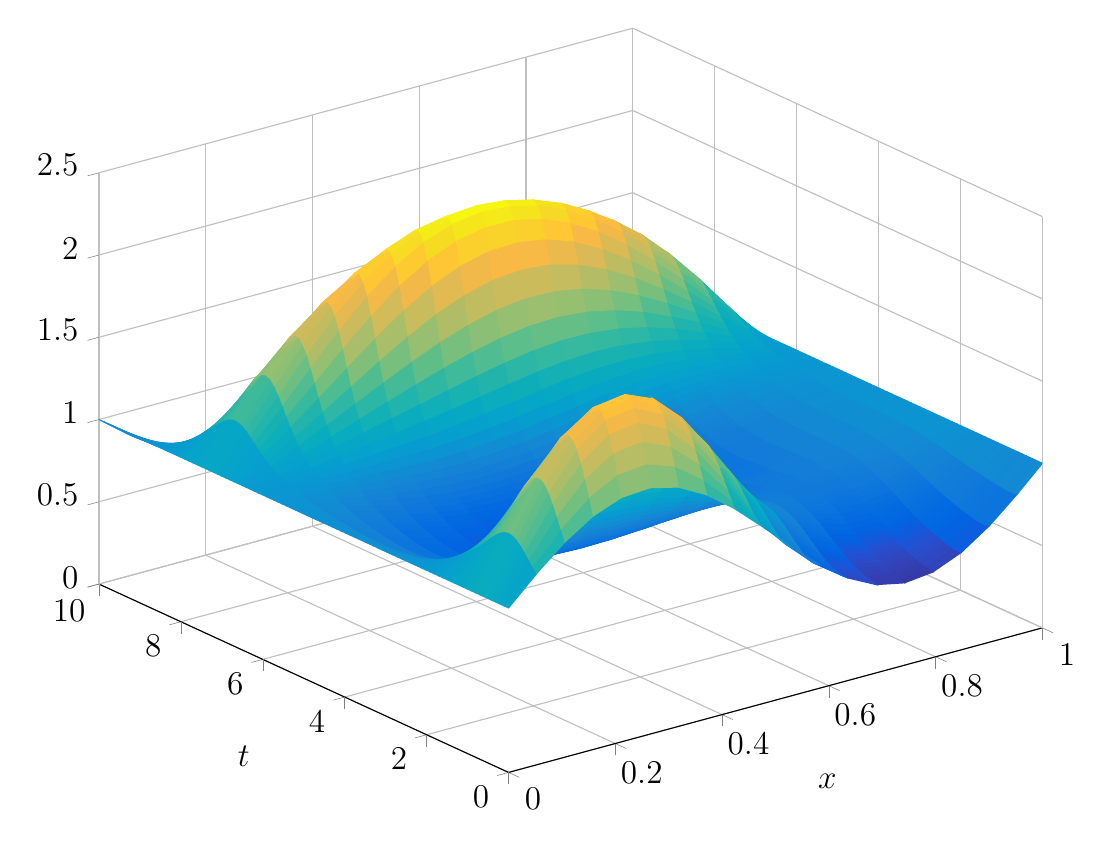
\begin{tikzpicture}

\begin{axis}[%
width=4.717in,
height=3.721in,
at={(0.791in,0.502in)},
scale only axis,
xmin=0,
xmax=1,
tick align=outside,
xlabel={$x$},
xlabel style = {font =\large},
xmajorgrids,
ymin=0,
ymax=10,
ylabel={$t$},
ylabel style = {font =\large},
ymajorgrids,
zmin=0,
zmax=2.5,
zmajorgrids,
view={-37.5}{30},
axis background/.style={fill=white},
axis x line*=bottom,
axis y line*=left,
axis z line*=left,
ticklabel style={font=\large},legend style={font=\large},title style={font=\large}
]

\addplot3[%
surf,
shader=flat,z buffer=sort,colormap={mymap}{[1pt] rgb(0pt)=(0.2081,0.1663,0.5292); rgb(1pt)=(0.211624,0.189781,0.577676); rgb(2pt)=(0.212252,0.213771,0.626971); rgb(3pt)=(0.2081,0.2386,0.677086); rgb(4pt)=(0.195905,0.264457,0.7279); rgb(5pt)=(0.170729,0.291938,0.779248); rgb(6pt)=(0.125271,0.324243,0.830271); rgb(7pt)=(0.0591333,0.359833,0.868333); rgb(8pt)=(0.0116952,0.38751,0.881957); rgb(9pt)=(0.00595714,0.408614,0.882843); rgb(10pt)=(0.0165143,0.4266,0.878633); rgb(11pt)=(0.0328524,0.443043,0.871957); rgb(12pt)=(0.0498143,0.458571,0.864057); rgb(13pt)=(0.0629333,0.47369,0.855438); rgb(14pt)=(0.0722667,0.488667,0.8467); rgb(15pt)=(0.0779429,0.503986,0.838371); rgb(16pt)=(0.0793476,0.520024,0.831181); rgb(17pt)=(0.0749429,0.537543,0.826271); rgb(18pt)=(0.0640571,0.556986,0.823957); rgb(19pt)=(0.0487714,0.577224,0.822829); rgb(20pt)=(0.0343429,0.596581,0.819852); rgb(21pt)=(0.0265,0.6137,0.8135); rgb(22pt)=(0.0238905,0.628662,0.803762); rgb(23pt)=(0.0230905,0.641786,0.791267); rgb(24pt)=(0.0227714,0.653486,0.776757); rgb(25pt)=(0.0266619,0.664195,0.760719); rgb(26pt)=(0.0383714,0.674271,0.743552); rgb(27pt)=(0.0589714,0.683757,0.725386); rgb(28pt)=(0.0843,0.692833,0.706167); rgb(29pt)=(0.113295,0.7015,0.685857); rgb(30pt)=(0.145271,0.709757,0.664629); rgb(31pt)=(0.180133,0.717657,0.642433); rgb(32pt)=(0.217829,0.725043,0.619262); rgb(33pt)=(0.258643,0.731714,0.595429); rgb(34pt)=(0.302171,0.737605,0.571186); rgb(35pt)=(0.348167,0.742433,0.547267); rgb(36pt)=(0.395257,0.7459,0.524443); rgb(37pt)=(0.44201,0.748081,0.503314); rgb(38pt)=(0.487124,0.749062,0.483976); rgb(39pt)=(0.530029,0.749114,0.466114); rgb(40pt)=(0.570857,0.748519,0.44939); rgb(41pt)=(0.609852,0.747314,0.433686); rgb(42pt)=(0.6473,0.7456,0.4188); rgb(43pt)=(0.683419,0.743476,0.404433); rgb(44pt)=(0.71841,0.741133,0.390476); rgb(45pt)=(0.752486,0.7384,0.376814); rgb(46pt)=(0.785843,0.735567,0.363271); rgb(47pt)=(0.818505,0.732733,0.34979); rgb(48pt)=(0.850657,0.7299,0.336029); rgb(49pt)=(0.882433,0.727433,0.3217); rgb(50pt)=(0.913933,0.725786,0.306276); rgb(51pt)=(0.944957,0.726114,0.288643); rgb(52pt)=(0.973895,0.731395,0.266648); rgb(53pt)=(0.993771,0.745457,0.240348); rgb(54pt)=(0.999043,0.765314,0.216414); rgb(55pt)=(0.995533,0.786057,0.196652); rgb(56pt)=(0.988,0.8066,0.179367); rgb(57pt)=(0.978857,0.827143,0.163314); rgb(58pt)=(0.9697,0.848138,0.147452); rgb(59pt)=(0.962586,0.870514,0.1309); rgb(60pt)=(0.958871,0.8949,0.113243); rgb(61pt)=(0.959824,0.921833,0.0948381); rgb(62pt)=(0.9661,0.951443,0.0755333); rgb(63pt)=(0.9763,0.9831,0.0538)},mesh/rows=20]
table[row sep=crcr, point meta=\thisrow{c}] {%
%
x	y	z	c\\
0	0	1	1\\
0	0.099	1	1\\
0	0.199	1	1\\
0	0.299	1	1\\
0	0.399	1	1\\
0	0.499	1	1\\
0	0.599	1	1\\
0	0.699	1	1\\
0	0.799	1	1\\
0	0.899	1	1\\
0	0.999	1	1\\
0	1.099	1	1\\
0	1.199	1	1\\
0	1.299	1	1\\
0	1.399	1	1\\
0	1.499	1	1\\
0	1.599	1	1\\
0	1.699	1	1\\
0	1.799	1	1\\
0	1.899	1	1\\
0	1.999	1	1\\
0	2.099	1	1\\
0	2.199	1	1\\
0	2.299	1	1\\
0	2.399	1	1\\
0	2.499	1	1\\
0	2.599	1	1\\
0	2.699	1	1\\
0	2.799	1	1\\
0	2.899	1	1\\
0	2.999	1	1\\
0	3.099	1	1\\
0	3.199	1	1\\
0	3.299	1	1\\
0	3.399	1	1\\
0	3.499	1	1\\
0	3.599	1	1\\
0	3.699	1	1\\
0	3.799	1	1\\
0	3.899	1	1\\
0	3.999	1	1\\
0	4.099	1	1\\
0	4.199	1	1\\
0	4.299	1	1\\
0	4.399	1	1\\
0	4.499	1	1\\
0	4.599	1	1\\
0	4.699	1	1\\
0	4.799	1	1\\
0	4.899	1	1\\
0	4.999	1	1\\
0	5.099	1	1\\
0	5.199	1	1\\
0	5.299	1	1\\
0	5.399	1	1\\
0	5.499	1	1\\
0	5.599	1	1\\
0	5.699	1	1\\
0	5.799	1	1\\
0	5.899	1	1\\
0	5.999	1	1\\
0	6.099	1	1\\
0	6.199	1	1\\
0	6.299	1	1\\
0	6.399	1	1\\
0	6.499	1	1\\
0	6.599	1	1\\
0	6.699	1	1\\
0	6.799	1	1\\
0	6.899	1	1\\
0	6.999	1	1\\
0	7.099	1	1\\
0	7.199	1	1\\
0	7.299	1	1\\
0	7.399	1	1\\
0	7.499	1	1\\
0	7.599	1	1\\
0	7.699	1	1\\
0	7.799	1	1\\
0	7.899	1	1\\
0	7.999	1	1\\
0	8.099	1	1\\
0	8.199	1	1\\
0	8.299	1	1\\
0	8.399	1	1\\
0	8.499	1	1\\
0	8.599	1	1\\
0	8.699	1	1\\
0	8.799	1	1\\
0	8.899	1	1\\
0	8.999	1	1\\
0	9.099	1	1\\
0	9.199	1	1\\
0	9.299	1	1\\
0	9.399	1	1\\
0	9.499	1	1\\
0	9.599	1	1\\
0	9.699	1	1\\
0	9.799	1	1\\
0	9.899	1	1\\
0	9.999	1	1\\
0.0529801324503311	0	1.16339	1.16339\\
0.0529801324503311	0.099	1.19453	1.19453\\
0.0529801324503311	0.199	1.22919	1.22919\\
0.0529801324503311	0.299	1.26365	1.26365\\
0.0529801324503311	0.399	1.29435	1.29435\\
0.0529801324503311	0.499	1.31786	1.31786\\
0.0529801324503311	0.599	1.33164	1.33164\\
0.0529801324503311	0.699	1.33466	1.33466\\
0.0529801324503311	0.799	1.3275	1.3275\\
0.0529801324503311	0.899	1.31185	1.31185\\
0.0529801324503311	0.999	1.28987	1.28987\\
0.0529801324503311	1.099	1.26375	1.26375\\
0.0529801324503311	1.199	1.23532	1.23532\\
0.0529801324503311	1.299	1.20603	1.20603\\
0.0529801324503311	1.399	1.17694	1.17694\\
0.0529801324503311	1.499	1.14875	1.14875\\
0.0529801324503311	1.599	1.12193	1.12193\\
0.0529801324503311	1.699	1.09676	1.09676\\
0.0529801324503311	1.799	1.07339	1.07339\\
0.0529801324503311	1.899	1.05187	1.05187\\
0.0529801324503311	1.999	1.0322	1.0322\\
0.0529801324503311	2.099	1.01433	1.01433\\
0.0529801324503311	2.199	0.998188	0.998188\\
0.0529801324503311	2.299	0.983695	0.983695\\
0.0529801324503311	2.399	0.970756	0.970756\\
0.0529801324503311	2.499	0.959277	0.959277\\
0.0529801324503311	2.599	0.949159	0.949159\\
0.0529801324503311	2.699	0.940309	0.940309\\
0.0529801324503311	2.799	0.932633	0.932633\\
0.0529801324503311	2.899	0.926042	0.926042\\
0.0529801324503311	2.999	0.920453	0.920453\\
0.0529801324503311	3.099	0.915784	0.915784\\
0.0529801324503311	3.199	0.911962	0.911962\\
0.0529801324503311	3.299	0.908915	0.908915\\
0.0529801324503311	3.399	0.90658	0.90658\\
0.0529801324503311	3.499	0.904896	0.904896\\
0.0529801324503311	3.599	0.903811	0.903811\\
0.0529801324503311	3.699	0.903275	0.903275\\
0.0529801324503311	3.799	0.903244	0.903244\\
0.0529801324503311	3.899	0.90368	0.90368\\
0.0529801324503311	3.999	0.904549	0.904549\\
0.0529801324503311	4.099	0.905822	0.905822\\
0.0529801324503311	4.199	0.907474	0.907474\\
0.0529801324503311	4.299	0.909486	0.909486\\
0.0529801324503311	4.399	0.91184	0.91184\\
0.0529801324503311	4.499	0.914526	0.914526\\
0.0529801324503311	4.599	0.917536	0.917536\\
0.0529801324503311	4.699	0.920867	0.920867\\
0.0529801324503311	4.799	0.92452	0.92452\\
0.0529801324503311	4.899	0.928502	0.928502\\
0.0529801324503311	4.999	0.932822	0.932822\\
0.0529801324503311	5.099	0.937499	0.937499\\
0.0529801324503311	5.199	0.942554	0.942554\\
0.0529801324503311	5.299	0.948016	0.948016\\
0.0529801324503311	5.399	0.953926	0.953926\\
0.0529801324503311	5.499	0.960329	0.960329\\
0.0529801324503311	5.599	0.967286	0.967286\\
0.0529801324503311	5.699	0.974872	0.974872\\
0.0529801324503311	5.799	0.983179	0.983179\\
0.0529801324503311	5.899	0.992322	0.992322\\
0.0529801324503311	5.999	1.00244	1.00244\\
0.0529801324503311	6.099	1.01371	1.01371\\
0.0529801324503311	6.199	1.02634	1.02634\\
0.0529801324503311	6.299	1.0406	1.0406\\
0.0529801324503311	6.399	1.05677	1.05677\\
0.0529801324503311	6.499	1.07517	1.07517\\
0.0529801324503311	6.599	1.0961	1.0961\\
0.0529801324503311	6.699	1.1197	1.1197\\
0.0529801324503311	6.799	1.14575	1.14575\\
0.0529801324503311	6.899	1.17336	1.17336\\
0.0529801324503311	6.999	1.20069	1.20069\\
0.0529801324503311	7.099	1.22501	1.22501\\
0.0529801324503311	7.199	1.24326	1.24326\\
0.0529801324503311	7.299	1.25303	1.25303\\
0.0529801324503311	7.399	1.25328	1.25328\\
0.0529801324503311	7.499	1.24444	1.24444\\
0.0529801324503311	7.599	1.22802	1.22802\\
0.0529801324503311	7.699	1.20595	1.20595\\
0.0529801324503311	7.799	1.1802	1.1802\\
0.0529801324503311	7.899	1.15244	1.15244\\
0.0529801324503311	7.999	1.124	1.124\\
0.0529801324503311	8.099	1.09586	1.09586\\
0.0529801324503311	8.199	1.06871	1.06871\\
0.0529801324503311	8.299	1.04302	1.04302\\
0.0529801324503311	8.399	1.01909	1.01909\\
0.0529801324503311	8.499	0.997073	0.997073\\
0.0529801324503311	8.599	0.977062	0.977062\\
0.0529801324503311	8.699	0.959069	0.959069\\
0.0529801324503311	8.799	0.94306	0.94306\\
0.0529801324503311	8.899	0.928966	0.928966\\
0.0529801324503311	8.999	0.916694	0.916694\\
0.0529801324503311	9.099	0.906134	0.906134\\
0.0529801324503311	9.199	0.897164	0.897164\\
0.0529801324503311	9.299	0.889655	0.889655\\
0.0529801324503311	9.399	0.883478	0.883478\\
0.0529801324503311	9.499	0.878507	0.878507\\
0.0529801324503311	9.599	0.874618	0.874618\\
0.0529801324503311	9.699	0.871697	0.871697\\
0.0529801324503311	9.799	0.869638	0.869638\\
0.0529801324503311	9.899	0.868343	0.868343\\
0.0529801324503311	9.999	0.867725	0.867725\\
0.105960264900662	0	1.30883	1.30883\\
0.105960264900662	0.099	1.37687	1.37687\\
0.105960264900662	0.199	1.4466	1.4466\\
0.105960264900662	0.299	1.51234	1.51234\\
0.105960264900662	0.399	1.56751	1.56751\\
0.105960264900662	0.499	1.60632	1.60632\\
0.105960264900662	0.599	1.62534	1.62534\\
0.105960264900662	0.699	1.62422	1.62422\\
0.105960264900662	0.799	1.60521	1.60521\\
0.105960264900662	0.899	1.57205	1.57205\\
0.105960264900662	0.999	1.52885	1.52885\\
0.105960264900662	1.099	1.47935	1.47935\\
0.105960264900662	1.199	1.42659	1.42659\\
0.105960264900662	1.299	1.37289	1.37289\\
0.105960264900662	1.399	1.31988	1.31988\\
0.105960264900662	1.499	1.26869	1.26869\\
0.105960264900662	1.599	1.22004	1.22004\\
0.105960264900662	1.699	1.17435	1.17435\\
0.105960264900662	1.799	1.13186	1.13186\\
0.105960264900662	1.899	1.09265	1.09265\\
0.105960264900662	1.999	1.05672	1.05672\\
0.105960264900662	2.099	1.02398	1.02398\\
0.105960264900662	2.199	0.994336	0.994336\\
0.105960264900662	2.299	0.967635	0.967635\\
0.105960264900662	2.399	0.943723	0.943723\\
0.105960264900662	2.499	0.922438	0.922438\\
0.105960264900662	2.599	0.903613	0.903613\\
0.105960264900662	2.699	0.887083	0.887083\\
0.105960264900662	2.799	0.872686	0.872686\\
0.105960264900662	2.899	0.860264	0.860264\\
0.105960264900662	2.999	0.849667	0.849667\\
0.105960264900662	3.099	0.840754	0.840754\\
0.105960264900662	3.199	0.833388	0.833388\\
0.105960264900662	3.299	0.827446	0.827446\\
0.105960264900662	3.399	0.822811	0.822811\\
0.105960264900662	3.499	0.819378	0.819378\\
0.105960264900662	3.599	0.817049	0.817049\\
0.105960264900662	3.699	0.815738	0.815738\\
0.105960264900662	3.799	0.815366	0.815366\\
0.105960264900662	3.899	0.815867	0.815867\\
0.105960264900662	3.999	0.81718	0.81718\\
0.105960264900662	4.099	0.819256	0.819256\\
0.105960264900662	4.199	0.822052	0.822052\\
0.105960264900662	4.299	0.825534	0.825534\\
0.105960264900662	4.399	0.829678	0.829678\\
0.105960264900662	4.499	0.834466	0.834466\\
0.105960264900662	4.599	0.839888	0.839888\\
0.105960264900662	4.699	0.845945	0.845945\\
0.105960264900662	4.799	0.852643	0.852643\\
0.105960264900662	4.899	0.860001	0.860001\\
0.105960264900662	4.999	0.868047	0.868047\\
0.105960264900662	5.099	0.876818	0.876818\\
0.105960264900662	5.199	0.886368	0.886368\\
0.105960264900662	5.299	0.896764	0.896764\\
0.105960264900662	5.399	0.90809	0.90809\\
0.105960264900662	5.499	0.920454	0.920454\\
0.105960264900662	5.599	0.933988	0.933988\\
0.105960264900662	5.699	0.948856	0.948856\\
0.105960264900662	5.799	0.965264	0.965264\\
0.105960264900662	5.899	0.983465	0.983465\\
0.105960264900662	5.999	1.00377	1.00377\\
0.105960264900662	6.099	1.02657	1.02657\\
0.105960264900662	6.199	1.05232	1.05232\\
0.105960264900662	6.299	1.08159	1.08159\\
0.105960264900662	6.399	1.115	1.115\\
0.105960264900662	6.499	1.15319	1.15319\\
0.105960264900662	6.599	1.19666	1.19666\\
0.105960264900662	6.699	1.2454	1.2454\\
0.105960264900662	6.799	1.29844	1.29844\\
0.105960264900662	6.899	1.35312	1.35312\\
0.105960264900662	6.999	1.40483	1.40483\\
0.105960264900662	7.099	1.4477	1.4477\\
0.105960264900662	7.199	1.47623	1.47623\\
0.105960264900662	7.299	1.48713	1.48713\\
0.105960264900662	7.399	1.48002	1.48002\\
0.105960264900662	7.499	1.45699	1.45699\\
0.105960264900662	7.599	1.42142	1.42142\\
0.105960264900662	7.699	1.37704	1.37704\\
0.105960264900662	7.799	1.32721	1.32721\\
0.105960264900662	7.899	1.2747	1.2747\\
0.105960264900662	7.999	1.22164	1.22164\\
0.105960264900662	8.099	1.16958	1.16958\\
0.105960264900662	8.199	1.1196	1.1196\\
0.105960264900662	8.299	1.07244	1.07244\\
0.105960264900662	8.399	1.02857	1.02857\\
0.105960264900662	8.499	0.988259	0.988259\\
0.105960264900662	8.599	0.951624	0.951624\\
0.105960264900662	8.699	0.918681	0.918681\\
0.105960264900662	8.799	0.889362	0.889362\\
0.105960264900662	8.899	0.863538	0.863538\\
0.105960264900662	8.999	0.841034	0.841034\\
0.105960264900662	9.099	0.821642	0.821642\\
0.105960264900662	9.199	0.805135	0.805135\\
0.105960264900662	9.299	0.791276	0.791276\\
0.105960264900662	9.399	0.779825	0.779825\\
0.105960264900662	9.499	0.770549	0.770549\\
0.105960264900662	9.599	0.763224	0.763224\\
0.105960264900662	9.699	0.75764	0.75764\\
0.105960264900662	9.799	0.753606	0.753606\\
0.105960264900662	9.899	0.750947	0.750947\\
0.105960264900662	9.999	0.749508	0.749508\\
0.158940397350993	0	1.42037	1.42037\\
0.158940397350993	0.099	1.52454	1.52454\\
0.158940397350993	0.199	1.62541	1.62541\\
0.158940397350993	0.299	1.71513	1.71513\\
0.158940397350993	0.399	1.78516	1.78516\\
0.158940397350993	0.499	1.82913	1.82913\\
0.158940397350993	0.599	1.8447	1.8447\\
0.158940397350993	0.699	1.8337	1.8337\\
0.158940397350993	0.799	1.80069	1.80069\\
0.158940397350993	0.899	1.75128	1.75128\\
0.158940397350993	0.999	1.69086	1.69086\\
0.158940397350993	1.099	1.62393	1.62393\\
0.158940397350993	1.199	1.55399	1.55399\\
0.158940397350993	1.299	1.48357	1.48357\\
0.158940397350993	1.399	1.41447	1.41447\\
0.158940397350993	1.499	1.34787	1.34787\\
0.158940397350993	1.599	1.28456	1.28456\\
0.158940397350993	1.699	1.22499	1.22499\\
0.158940397350993	1.799	1.16943	1.16943\\
0.158940397350993	1.899	1.11798	1.11798\\
0.158940397350993	1.999	1.07064	1.07064\\
0.158940397350993	2.099	1.02733	1.02733\\
0.158940397350993	2.199	0.987943	0.987943\\
0.158940397350993	2.299	0.952316	0.952316\\
0.158940397350993	2.399	0.920274	0.920274\\
0.158940397350993	2.499	0.891629	0.891629\\
0.158940397350993	2.599	0.866182	0.866182\\
0.158940397350993	2.699	0.843732	0.843732\\
0.158940397350993	2.799	0.824079	0.824079\\
0.158940397350993	2.899	0.807027	0.807027\\
0.158940397350993	2.999	0.792383	0.792383\\
0.158940397350993	3.099	0.779966	0.779966\\
0.158940397350993	3.199	0.769602	0.769602\\
0.158940397350993	3.299	0.761129	0.761129\\
0.158940397350993	3.399	0.754397	0.754397\\
0.158940397350993	3.499	0.749267	0.749267\\
0.158940397350993	3.599	0.745615	0.745615\\
0.158940397350993	3.699	0.743328	0.743328\\
0.158940397350993	3.799	0.742307	0.742307\\
0.158940397350993	3.899	0.742465	0.742465\\
0.158940397350993	3.999	0.743726	0.743726\\
0.158940397350993	4.099	0.746029	0.746029\\
0.158940397350993	4.199	0.749322	0.749322\\
0.158940397350993	4.299	0.753568	0.753568\\
0.158940397350993	4.399	0.758737	0.758737\\
0.158940397350993	4.499	0.764815	0.764815\\
0.158940397350993	4.599	0.771798	0.771798\\
0.158940397350993	4.699	0.779693	0.779693\\
0.158940397350993	4.799	0.788522	0.788522\\
0.158940397350993	4.899	0.798322	0.798322\\
0.158940397350993	4.999	0.809144	0.809144\\
0.158940397350993	5.099	0.821058	0.821058\\
0.158940397350993	5.199	0.834155	0.834155\\
0.158940397350993	5.299	0.84855	0.84855\\
0.158940397350993	5.399	0.864389	0.864389\\
0.158940397350993	5.499	0.881853	0.881853\\
0.158940397350993	5.599	0.901168	0.901168\\
0.158940397350993	5.699	0.922614	0.922614\\
0.158940397350993	5.799	0.946541	0.946541\\
0.158940397350993	5.899	0.973381	0.973381\\
0.158940397350993	5.999	1.00367	1.00367\\
0.158940397350993	6.099	1.03808	1.03808\\
0.158940397350993	6.199	1.07739	1.07739\\
0.158940397350993	6.299	1.12255	1.12255\\
0.158940397350993	6.399	1.17458	1.17458\\
0.158940397350993	6.499	1.23439	1.23439\\
0.158940397350993	6.599	1.30245	1.30245\\
0.158940397350993	6.699	1.37806	1.37806\\
0.158940397350993	6.799	1.45834	1.45834\\
0.158940397350993	6.899	1.5374	1.5374\\
0.158940397350993	6.999	1.60677	1.60677\\
0.158940397350993	7.099	1.65766	1.65766\\
0.158940397350993	7.199	1.68399	1.68399\\
0.158940397350993	7.299	1.68417	1.68417\\
0.158940397350993	7.399	1.66059	1.66059\\
0.158940397350993	7.499	1.61793	1.61793\\
0.158940397350993	7.599	1.56147	1.56147\\
0.158940397350993	7.699	1.49606	1.49606\\
0.158940397350993	7.799	1.42569	1.42569\\
0.158940397350993	7.899	1.35344	1.35344\\
0.158940397350993	7.999	1.2816	1.2816\\
0.158940397350993	8.099	1.2118	1.2118\\
0.158940397350993	8.199	1.14519	1.14519\\
0.158940397350993	8.299	1.08256	1.08256\\
0.158940397350993	8.399	1.0244	1.0244\\
0.158940397350993	8.499	0.971012	0.971012\\
0.158940397350993	8.599	0.922515	0.922515\\
0.158940397350993	8.699	0.878915	0.878915\\
0.158940397350993	8.799	0.840114	0.840114\\
0.158940397350993	8.899	0.805934	0.805934\\
0.158940397350993	8.999	0.776136	0.776136\\
0.158940397350993	9.099	0.75044	0.75044\\
0.158940397350993	9.199	0.728535	0.728535\\
0.158940397350993	9.299	0.710099	0.710099\\
0.158940397350993	9.399	0.69481	0.69481\\
0.158940397350993	9.499	0.682352	0.682352\\
0.158940397350993	9.599	0.672426	0.672426\\
0.158940397350993	9.699	0.664755	0.664755\\
0.158940397350993	9.799	0.659087	0.659087\\
0.158940397350993	9.899	0.655193	0.655193\\
0.158940397350993	9.999	0.652874	0.652874\\
0.211920529801325	0	1.48576	1.48576\\
0.211920529801325	0.099	1.61445	1.61445\\
0.211920529801325	0.199	1.73549	1.73549\\
0.211920529801325	0.299	1.83894	1.83894\\
0.211920529801325	0.399	1.91542	1.91542\\
0.211920529801325	0.499	1.95912	1.95912\\
0.211920529801325	0.599	1.96936	1.96936\\
0.211920529801325	0.699	1.9499	1.9499\\
0.211920529801325	0.799	1.90697	1.90697\\
0.211920529801325	0.899	1.84726	1.84726\\
0.211920529801325	0.999	1.77672	1.77672\\
0.211920529801325	1.099	1.70009	1.70009\\
0.211920529801325	1.199	1.62089	1.62089\\
0.211920529801325	1.299	1.54163	1.54163\\
0.211920529801325	1.399	1.46403	1.46403\\
0.211920529801325	1.499	1.38924	1.38924\\
0.211920529801325	1.599	1.31801	1.31801\\
0.211920529801325	1.699	1.25079	1.25079\\
0.211920529801325	1.799	1.18786	1.18786\\
0.211920529801325	1.899	1.12932	1.12932\\
0.211920529801325	1.999	1.0752	1.0752\\
0.211920529801325	2.099	1.02546	1.02546\\
0.211920529801325	2.199	0.979993	0.979993\\
0.211920529801325	2.299	0.93867	0.93867\\
0.211920529801325	2.399	0.901329	0.901329\\
0.211920529801325	2.499	0.867786	0.867786\\
0.211920529801325	2.599	0.837845	0.837845\\
0.211920529801325	2.699	0.811301	0.811301\\
0.211920529801325	2.799	0.787942	0.787942\\
0.211920529801325	2.899	0.767557	0.767557\\
0.211920529801325	2.999	0.749938	0.749938\\
0.211920529801325	3.099	0.734884	0.734884\\
0.211920529801325	3.199	0.7222	0.7222\\
0.211920529801325	3.299	0.711703	0.711703\\
0.211920529801325	3.399	0.703225	0.703225\\
0.211920529801325	3.499	0.696607	0.696607\\
0.211920529801325	3.599	0.691709	0.691709\\
0.211920529801325	3.699	0.688403	0.688403\\
0.211920529801325	3.799	0.686578	0.686578\\
0.211920529801325	3.899	0.686135	0.686135\\
0.211920529801325	3.999	0.686993	0.686993\\
0.211920529801325	4.099	0.689084	0.689084\\
0.211920529801325	4.199	0.692354	0.692354\\
0.211920529801325	4.299	0.696766	0.696766\\
0.211920529801325	4.399	0.702294	0.702294\\
0.211920529801325	4.499	0.70893	0.70893\\
0.211920529801325	4.599	0.716678	0.716678\\
0.211920529801325	4.699	0.725562	0.725562\\
0.211920529801325	4.799	0.735619	0.735619\\
0.211920529801325	4.899	0.74691	0.74691\\
0.211920529801325	4.999	0.759514	0.759514\\
0.211920529801325	5.099	0.773539	0.773539\\
0.211920529801325	5.199	0.789121	0.789121\\
0.211920529801325	5.299	0.806432	0.806432\\
0.211920529801325	5.399	0.825689	0.825689\\
0.211920529801325	5.499	0.847161	0.847161\\
0.211920529801325	5.599	0.871188	0.871188\\
0.211920529801325	5.699	0.89819	0.89819\\
0.211920529801325	5.799	0.928697	0.928697\\
0.211920529801325	5.899	0.963368	0.963368\\
0.211920529801325	5.999	1.00303	1.00303\\
0.211920529801325	6.099	1.04869	1.04869\\
0.211920529801325	6.199	1.10157	1.10157\\
0.211920529801325	6.299	1.16308	1.16308\\
0.211920529801325	6.399	1.23466	1.23466\\
0.211920529801325	6.499	1.31744	1.31744\\
0.211920529801325	6.599	1.41144	1.41144\\
0.211920529801325	6.699	1.51429	1.51429\\
0.211920529801325	6.799	1.61974	1.61974\\
0.211920529801325	6.899	1.71726	1.71726\\
0.211920529801325	6.999	1.79432	1.79432\\
0.211920529801325	7.099	1.84096	1.84096\\
0.211920529801325	7.199	1.85331	1.85331\\
0.211920529801325	7.299	1.83377	1.83377\\
0.211920529801325	7.399	1.78841	1.78841\\
0.211920529801325	7.499	1.72435	1.72435\\
0.211920529801325	7.599	1.64805	1.64805\\
0.211920529801325	7.699	1.56473	1.56473\\
0.211920529801325	7.799	1.47831	1.47831\\
0.211920529801325	7.899	1.39166	1.39166\\
0.211920529801325	7.999	1.3068	1.3068\\
0.211920529801325	8.099	1.22517	1.22517\\
0.211920529801325	8.199	1.14777	1.14777\\
0.211920529801325	8.299	1.07527	1.07527\\
0.211920529801325	8.399	1.00812	1.00812\\
0.211920529801325	8.499	0.946558	0.946558\\
0.211920529801325	8.599	0.890702	0.890702\\
0.211920529801325	8.699	0.840527	0.840527\\
0.211920529801325	8.799	0.795903	0.795903\\
0.211920529801325	8.899	0.756615	0.756615\\
0.211920529801325	8.999	0.722376	0.722376\\
0.211920529801325	9.099	0.692849	0.692849\\
0.211920529801325	9.199	0.667666	0.667666\\
0.211920529801325	9.299	0.646445	0.646445\\
0.211920529801325	9.399	0.628802	0.628802\\
0.211920529801325	9.499	0.614367	0.614367\\
0.211920529801325	9.599	0.60279	0.60279\\
0.211920529801325	9.699	0.593748	0.593748\\
0.211920529801325	9.799	0.586951	0.586951\\
0.211920529801325	9.899	0.582138	0.582138\\
0.211920529801325	9.999	0.579081	0.579081\\
0.264900662251656	0	1.49781	1.49781\\
0.264900662251656	0.099	1.6313	1.6313\\
0.264900662251656	0.199	1.75622	1.75622\\
0.264900662251656	0.299	1.86226	1.86226\\
0.264900662251656	0.399	1.9401	1.9401\\
0.264900662251656	0.499	1.98417	1.98417\\
0.264900662251656	0.599	1.99411	1.99411\\
0.264900662251656	0.699	1.97396	1.97396\\
0.264900662251656	0.799	1.9301	1.9301\\
0.264900662251656	0.899	1.86931	1.86931\\
0.264900662251656	0.999	1.79753	1.79753\\
0.264900662251656	1.099	1.7195	1.7195\\
0.264900662251656	1.199	1.6387	1.6387\\
0.264900662251656	1.299	1.55763	1.55763\\
0.264900662251656	1.399	1.478	1.478\\
0.264900662251656	1.499	1.40095	1.40095\\
0.264900662251656	1.599	1.32726	1.32726\\
0.264900662251656	1.699	1.25739	1.25739\\
0.264900662251656	1.799	1.19165	1.19165\\
0.264900662251656	1.899	1.13018	1.13018\\
0.264900662251656	1.999	1.07307	1.07307\\
0.264900662251656	2.099	1.0203	1.0203\\
0.264900662251656	2.199	0.971812	0.971812\\
0.264900662251656	2.299	0.927523	0.927523\\
0.264900662251656	2.399	0.887301	0.887301\\
0.264900662251656	2.499	0.850993	0.850993\\
0.264900662251656	2.599	0.818425	0.818425\\
0.264900662251656	2.699	0.789408	0.789408\\
0.264900662251656	2.799	0.763742	0.763742\\
0.264900662251656	2.899	0.74122	0.74122\\
0.264900662251656	2.999	0.721636	0.721636\\
0.264900662251656	3.099	0.704784	0.704784\\
0.264900662251656	3.199	0.690466	0.690466\\
0.264900662251656	3.299	0.678494	0.678494\\
0.264900662251656	3.399	0.668689	0.668689\\
0.264900662251656	3.499	0.660887	0.660887\\
0.264900662251656	3.599	0.654939	0.654939\\
0.264900662251656	3.699	0.650712	0.650712\\
0.264900662251656	3.799	0.648089	0.648089\\
0.264900662251656	3.899	0.646967	0.646967\\
0.264900662251656	3.999	0.647263	0.647263\\
0.264900662251656	4.099	0.648909	0.648909\\
0.264900662251656	4.199	0.651851	0.651851\\
0.264900662251656	4.299	0.656055	0.656055\\
0.264900662251656	4.399	0.661503	0.661503\\
0.264900662251656	4.499	0.668191	0.668191\\
0.264900662251656	4.599	0.676138	0.676138\\
0.264900662251656	4.699	0.68538	0.68538\\
0.264900662251656	4.799	0.695975	0.695975\\
0.264900662251656	4.899	0.708005	0.708005\\
0.264900662251656	4.999	0.721581	0.721581\\
0.264900662251656	5.099	0.736847	0.736847\\
0.264900662251656	5.199	0.753987	0.753987\\
0.264900662251656	5.299	0.773231	0.773231\\
0.264900662251656	5.399	0.794872	0.794872\\
0.264900662251656	5.499	0.819275	0.819275\\
0.264900662251656	5.599	0.846902	0.846902\\
0.264900662251656	5.699	0.878331	0.878331\\
0.264900662251656	5.799	0.914295	0.914295\\
0.264900662251656	5.899	0.955715	0.955715\\
0.264900662251656	5.999	1.00375	1.00375\\
0.264900662251656	6.099	1.05982	1.05982\\
0.264900662251656	6.199	1.12566	1.12566\\
0.264900662251656	6.299	1.2032	1.2032\\
0.264900662251656	6.399	1.2943	1.2943\\
0.264900662251656	6.499	1.40008	1.40008\\
0.264900662251656	6.599	1.51953	1.51953\\
0.264900662251656	6.699	1.64748	1.64748\\
0.264900662251656	6.799	1.77297	1.77297\\
0.264900662251656	6.899	1.88033	1.88033\\
0.264900662251656	6.999	1.95439	1.95439\\
0.264900662251656	7.099	1.98679	1.98679\\
0.264900662251656	7.199	1.9782	1.9782\\
0.264900662251656	7.299	1.93568	1.93568\\
0.264900662251656	7.399	1.86843	1.86843\\
0.264900662251656	7.499	1.785	1.785\\
0.264900662251656	7.599	1.69222	1.69222\\
0.264900662251656	7.699	1.59506	1.59506\\
0.264900662251656	7.799	1.49703	1.49703\\
0.264900662251656	7.899	1.40057	1.40057\\
0.264900662251656	7.999	1.30731	1.30731\\
0.264900662251656	8.099	1.2184	1.2184\\
0.264900662251656	8.199	1.13462	1.13462\\
0.264900662251656	8.299	1.05648	1.05648\\
0.264900662251656	8.399	0.984331	0.984331\\
0.264900662251656	8.499	0.918348	0.918348\\
0.264900662251656	8.599	0.858587	0.858587\\
0.264900662251656	8.699	0.804986	0.804986\\
0.264900662251656	8.799	0.75738	0.75738\\
0.264900662251656	8.899	0.715517	0.715517\\
0.264900662251656	8.999	0.679071	0.679071\\
0.264900662251656	9.099	0.647664	0.647664\\
0.264900662251656	9.199	0.620888	0.620888\\
0.264900662251656	9.299	0.598316	0.598316\\
0.264900662251656	9.399	0.579529	0.579529\\
0.264900662251656	9.499	0.564119	0.564119\\
0.264900662251656	9.599	0.551708	0.551708\\
0.264900662251656	9.699	0.541946	0.541946\\
0.264900662251656	9.799	0.534521	0.534521\\
0.264900662251656	9.899	0.529154	0.529154\\
0.264900662251656	9.999	0.525605	0.525605\\
0.317880794701987	0	1.45521	1.45521\\
0.317880794701987	0.099	1.57214	1.57214\\
0.317880794701987	0.199	1.68367	1.68367\\
0.317880794701987	0.299	1.78143	1.78143\\
0.317880794701987	0.399	1.8569	1.8569\\
0.317880794701987	0.499	1.90404	1.90404\\
0.317880794701987	0.599	1.92096	1.92096\\
0.317880794701987	0.699	1.90989	1.90989\\
0.317880794701987	0.799	1.87569	1.87569\\
0.317880794701987	0.899	1.82412	1.82412\\
0.317880794701987	0.999	1.7606	1.7606\\
0.317880794701987	1.099	1.68966	1.68966\\
0.317880794701987	1.199	1.61476	1.61476\\
0.317880794701987	1.299	1.53848	1.53848\\
0.317880794701987	1.399	1.46265	1.46265\\
0.317880794701987	1.499	1.38853	1.38853\\
0.317880794701987	1.599	1.317	1.317\\
0.317880794701987	1.699	1.24865	1.24865\\
0.317880794701987	1.799	1.18387	1.18387\\
0.317880794701987	1.899	1.1229	1.1229\\
0.317880794701987	1.999	1.06588	1.06588\\
0.317880794701987	2.099	1.01287	1.01287\\
0.317880794701987	2.199	0.963896	0.963896\\
0.317880794701987	2.299	0.918909	0.918909\\
0.317880794701987	2.399	0.877833	0.877833\\
0.317880794701987	2.499	0.840559	0.840559\\
0.317880794701987	2.599	0.806953	0.806953\\
0.317880794701987	2.699	0.776856	0.776856\\
0.317880794701987	2.799	0.750095	0.750095\\
0.317880794701987	2.899	0.726484	0.726484\\
0.317880794701987	2.999	0.705832	0.705832\\
0.317880794701987	3.099	0.687945	0.687945\\
0.317880794701987	3.199	0.672633	0.672633\\
0.317880794701987	3.299	0.659712	0.659712\\
0.317880794701987	3.399	0.649009	0.649009\\
0.317880794701987	3.499	0.640362	0.640362\\
0.317880794701987	3.599	0.633622	0.633622\\
0.317880794701987	3.699	0.628658	0.628658\\
0.317880794701987	3.799	0.625352	0.625352\\
0.317880794701987	3.899	0.623606	0.623606\\
0.317880794701987	3.999	0.623336	0.623336\\
0.317880794701987	4.099	0.624475	0.624475\\
0.317880794701987	4.199	0.626977	0.626977\\
0.317880794701987	4.299	0.63081	0.63081\\
0.317880794701987	4.399	0.635962	0.635962\\
0.317880794701987	4.499	0.642439	0.642439\\
0.317880794701987	4.599	0.65027	0.65027\\
0.317880794701987	4.699	0.659505	0.659505\\
0.317880794701987	4.799	0.670217	0.670217\\
0.317880794701987	4.899	0.682512	0.682512\\
0.317880794701987	4.999	0.696528	0.696528\\
0.317880794701987	5.099	0.712441	0.712441\\
0.317880794701987	5.199	0.730479	0.730479\\
0.317880794701987	5.299	0.75093	0.75093\\
0.317880794701987	5.399	0.774155	0.774155\\
0.317880794701987	5.499	0.800615	0.800615\\
0.317880794701987	5.599	0.830889	0.830889\\
0.317880794701987	5.699	0.865714	0.865714\\
0.317880794701987	5.799	0.906028	0.906028\\
0.317880794701987	5.899	0.953022	0.953022\\
0.317880794701987	5.999	1.0082	1.0082\\
0.317880794701987	6.099	1.07343	1.07343\\
0.317880794701987	6.199	1.15094	1.15094\\
0.317880794701987	6.299	1.24318	1.24318\\
0.317880794701987	6.399	1.35235	1.35235\\
0.317880794701987	6.499	1.47923	1.47923\\
0.317880794701987	6.599	1.62112	1.62112\\
0.317880794701987	6.699	1.76916	1.76916\\
0.317880794701987	6.799	1.90714	1.90714\\
0.317880794701987	6.899	2.01521	2.01521\\
0.317880794701987	6.999	2.07803	2.07803\\
0.317880794701987	7.099	2.09119	2.09119\\
0.317880794701987	7.199	2.06053	2.06053\\
0.317880794701987	7.299	1.99688	1.99688\\
0.317880794701987	7.399	1.91127	1.91127\\
0.317880794701987	7.499	1.8127	1.8127\\
0.317880794701987	7.599	1.70771	1.70771\\
0.317880794701987	7.699	1.60081	1.60081\\
0.317880794701987	7.799	1.49501	1.49501\\
0.317880794701987	7.899	1.39229	1.39229\\
0.317880794701987	7.999	1.29397	1.29397\\
0.317880794701987	8.099	1.20092	1.20092\\
0.317880794701987	8.199	1.11373	1.11373\\
0.317880794701987	8.299	1.03276	1.03276\\
0.317880794701987	8.399	0.958251	0.958251\\
0.317880794701987	8.499	0.890306	0.890306\\
0.317880794701987	8.599	0.828917	0.828917\\
0.317880794701987	8.699	0.773973	0.773973\\
0.317880794701987	8.799	0.725268	0.725268\\
0.317880794701987	8.899	0.68251	0.68251\\
0.317880794701987	8.999	0.645341	0.645341\\
0.317880794701987	9.099	0.613351	0.613351\\
0.317880794701987	9.199	0.5861	0.5861\\
0.317880794701987	9.299	0.563139	0.563139\\
0.317880794701987	9.399	0.544023	0.544023\\
0.317880794701987	9.499	0.528326	0.528326\\
0.317880794701987	9.599	0.515654	0.515654\\
0.317880794701987	9.699	0.505644	0.505644\\
0.317880794701987	9.799	0.497973	0.497973\\
0.317880794701987	9.899	0.492359	0.492359\\
0.317880794701987	9.999	0.488554	0.488554\\
0.370860927152318	0	1.36263	1.36263\\
0.370860927152318	0.099	1.44723	1.44723\\
0.370860927152318	0.199	1.5321	1.5321\\
0.370860927152318	0.299	1.61196	1.61196\\
0.370860927152318	0.399	1.68004	1.68004\\
0.370860927152318	0.499	1.72998	1.72998\\
0.370860927152318	0.599	1.75777	1.75777\\
0.370860927152318	0.699	1.76262	1.76262\\
0.370860927152318	0.799	1.74653	1.74653\\
0.370860927152318	0.899	1.71317	1.71317\\
0.370860927152318	0.999	1.6667	1.6667\\
0.370860927152318	1.099	1.61101	1.61101\\
0.370860927152318	1.199	1.54941	1.54941\\
0.370860927152318	1.299	1.48451	1.48451\\
0.370860927152318	1.399	1.41829	1.41829\\
0.370860927152318	1.499	1.35224	1.35224\\
0.370860927152318	1.599	1.28743	1.28743\\
0.370860927152318	1.699	1.22464	1.22464\\
0.370860927152318	1.799	1.16442	1.16442\\
0.370860927152318	1.899	1.10716	1.10716\\
0.370860927152318	1.999	1.05313	1.05313\\
0.370860927152318	2.099	1.00249	1.00249\\
0.370860927152318	2.199	0.955341	0.955341\\
0.370860927152318	2.299	0.911734	0.911734\\
0.370860927152318	2.399	0.871657	0.871657\\
0.370860927152318	2.499	0.835064	0.835064\\
0.370860927152318	2.599	0.801871	0.801871\\
0.370860927152318	2.699	0.771968	0.771968\\
0.370860927152318	2.799	0.745223	0.745223\\
0.370860927152318	2.899	0.721485	0.721485\\
0.370860927152318	2.999	0.700593	0.700593\\
0.370860927152318	3.099	0.682378	0.682378\\
0.370860927152318	3.199	0.666673	0.666673\\
0.370860927152318	3.299	0.65331	0.65331\\
0.370860927152318	3.399	0.642132	0.642132\\
0.370860927152318	3.499	0.632987	0.632987\\
0.370860927152318	3.599	0.62574	0.62574\\
0.370860927152318	3.699	0.620265	0.620265\\
0.370860927152318	3.799	0.616453	0.616453\\
0.370860927152318	3.899	0.614212	0.614212\\
0.370860927152318	3.999	0.613464	0.613464\\
0.370860927152318	4.099	0.614149	0.614149\\
0.370860927152318	4.199	0.616226	0.616226\\
0.370860927152318	4.299	0.61967	0.61967\\
0.370860927152318	4.399	0.624476	0.624476\\
0.370860927152318	4.499	0.63066	0.63066\\
0.370860927152318	4.599	0.638259	0.638259\\
0.370860927152318	4.699	0.647335	0.647335\\
0.370860927152318	4.799	0.657978	0.657978\\
0.370860927152318	4.899	0.67031	0.67031\\
0.370860927152318	4.999	0.684491	0.684491\\
0.370860927152318	5.099	0.700729	0.700729\\
0.370860927152318	5.199	0.719287	0.719287\\
0.370860927152318	5.299	0.7405	0.7405\\
0.370860927152318	5.399	0.764792	0.764792\\
0.370860927152318	5.499	0.792702	0.792702\\
0.370860927152318	5.599	0.824915	0.824915\\
0.370860927152318	5.699	0.862309	0.862309\\
0.370860927152318	5.799	0.906003	0.906003\\
0.370860927152318	5.899	0.957432	0.957432\\
0.370860927152318	5.999	1.01841	1.01841\\
0.370860927152318	6.099	1.09119	1.09119\\
0.370860927152318	6.199	1.17843	1.17843\\
0.370860927152318	6.299	1.283	1.283\\
0.370860927152318	6.399	1.40716	1.40716\\
0.370860927152318	6.499	1.55105	1.55105\\
0.370860927152318	6.599	1.70981	1.70981\\
0.370860927152318	6.699	1.87064	1.87064\\
0.370860927152318	6.799	2.01288	2.01288\\
0.370860927152318	6.899	2.11453	2.11453\\
0.370860927152318	6.999	2.16231	2.16231\\
0.370860927152318	7.099	2.15645	2.15645\\
0.370860927152318	7.199	2.10698	2.10698\\
0.370860927152318	7.299	2.02698	2.02698\\
0.370860927152318	7.399	1.92811	1.92811\\
0.370860927152318	7.499	1.81917	1.81917\\
0.370860927152318	7.599	1.7062	1.7062\\
0.370860927152318	7.699	1.59319	1.59319\\
0.370860927152318	7.799	1.48271	1.48271\\
0.370860927152318	7.899	1.37643	1.37643\\
0.370860927152318	7.999	1.27539	1.27539\\
0.370860927152318	8.099	1.18029	1.18029\\
0.370860927152318	8.199	1.09157	1.09157\\
0.370860927152318	8.299	1.00949	1.00949\\
0.370860927152318	8.399	0.934206	0.934206\\
0.370860927152318	8.499	0.865743	0.865743\\
0.370860927152318	8.599	0.804042	0.804042\\
0.370860927152318	8.699	0.748944	0.748944\\
0.370860927152318	8.799	0.700201	0.700201\\
0.370860927152318	8.899	0.65749	0.65749\\
0.370860927152318	8.999	0.620421	0.620421\\
0.370860927152318	9.099	0.588561	0.588561\\
0.370860927152318	9.199	0.561452	0.561452\\
0.370860927152318	9.299	0.538626	0.538626\\
0.370860927152318	9.399	0.519629	0.519629\\
0.370860927152318	9.499	0.504026	0.504026\\
0.370860927152318	9.599	0.491416	0.491416\\
0.370860927152318	9.699	0.481433	0.481433\\
0.370860927152318	9.799	0.473753	0.473753\\
0.370860927152318	9.899	0.468091	0.468091\\
0.370860927152318	9.999	0.464202	0.464202\\
0.423841059602649	0	1.23023	1.23023\\
0.423841059602649	0.099	1.2773	1.2773\\
0.423841059602649	0.199	1.33034	1.33034\\
0.423841059602649	0.299	1.38662	1.38662\\
0.423841059602649	0.399	1.4415	1.4415\\
0.423841059602649	0.499	1.48945	1.48945\\
0.423841059602649	0.599	1.52548	1.52548\\
0.423841059602649	0.699	1.54634	1.54634\\
0.423841059602649	0.799	1.55102	1.55102\\
0.423841059602649	0.899	1.54044	1.54044\\
0.423841059602649	0.999	1.51672	1.51672\\
0.423841059602649	1.099	1.48251	1.48251\\
0.423841059602649	1.199	1.44047	1.44047\\
0.423841059602649	1.299	1.39295	1.39295\\
0.423841059602649	1.399	1.34197	1.34197\\
0.423841059602649	1.499	1.28913	1.28913\\
0.423841059602649	1.599	1.2357	1.2357\\
0.423841059602649	1.699	1.18266	1.18266\\
0.423841059602649	1.799	1.13077	1.13077\\
0.423841059602649	1.899	1.08059	1.08059\\
0.423841059602649	1.999	1.03256	1.03256\\
0.423841059602649	2.099	0.986972	0.986972\\
0.423841059602649	2.199	0.944061	0.944061\\
0.423841059602649	2.299	0.903971	0.903971\\
0.423841059602649	2.399	0.866788	0.866788\\
0.423841059602649	2.499	0.832547	0.832547\\
0.423841059602649	2.599	0.801237	0.801237\\
0.423841059602649	2.699	0.772815	0.772815\\
0.423841059602649	2.799	0.747204	0.747204\\
0.423841059602649	2.899	0.724306	0.724306\\
0.423841059602649	2.999	0.704006	0.704006\\
0.423841059602649	3.099	0.686175	0.686175\\
0.423841059602649	3.199	0.670681	0.670681\\
0.423841059602649	3.299	0.65739	0.65739\\
0.423841059602649	3.399	0.646167	0.646167\\
0.423841059602649	3.499	0.636888	0.636888\\
0.423841059602649	3.599	0.629433	0.629433\\
0.423841059602649	3.699	0.623698	0.623698\\
0.423841059602649	3.799	0.619587	0.619587\\
0.423841059602649	3.899	0.61702	0.61702\\
0.423841059602649	3.999	0.615932	0.615932\\
0.423841059602649	4.099	0.616273	0.616273\\
0.423841059602649	4.199	0.61801	0.61801\\
0.423841059602649	4.299	0.621129	0.621129\\
0.423841059602649	4.399	0.625633	0.625633\\
0.423841059602649	4.499	0.631547	0.631547\\
0.423841059602649	4.599	0.638918	0.638918\\
0.423841059602649	4.699	0.64782	0.64782\\
0.423841059602649	4.799	0.658354	0.658354\\
0.423841059602649	4.899	0.670658	0.670658\\
0.423841059602649	4.999	0.684912	0.684912\\
0.423841059602649	5.099	0.701344	0.701344\\
0.423841059602649	5.199	0.720247	0.720247\\
0.423841059602649	5.299	0.741992	0.741992\\
0.423841059602649	5.399	0.76705	0.76705\\
0.423841059602649	5.499	0.796022	0.796022\\
0.423841059602649	5.599	0.829674	0.829674\\
0.423841059602649	5.699	0.868987	0.868987\\
0.423841059602649	5.799	0.915218	0.915218\\
0.423841059602649	5.899	0.969977	0.969977\\
0.423841059602649	5.999	1.0353	1.0353\\
0.423841059602649	6.099	1.1137	1.1137\\
0.423841059602649	6.199	1.20811	1.20811\\
0.423841059602649	6.299	1.32153	1.32153\\
0.423841059602649	6.399	1.45608	1.45608\\
0.423841059602649	6.499	1.61092	1.61092\\
0.423841059602649	6.599	1.77907	1.77907\\
0.423841059602649	6.699	1.94458	1.94458\\
0.423841059602649	6.799	2.08415	2.08415\\
0.423841059602649	6.899	2.17576	2.17576\\
0.423841059602649	6.999	2.20912	2.20912\\
0.423841059602649	7.099	2.1882	2.1882\\
0.423841059602649	7.199	2.12549	2.12549\\
0.423841059602649	7.299	2.03494	2.03494\\
0.423841059602649	7.399	1.92811	1.92811\\
0.423841059602649	7.499	1.81329	1.81329\\
0.423841059602649	7.599	1.69604	1.69604\\
0.423841059602649	7.699	1.57994	1.57994\\
0.423841059602649	7.799	1.46727	1.46727\\
0.423841059602649	7.899	1.35944	1.35944\\
0.423841059602649	7.999	1.25738	1.25738\\
0.423841059602649	8.099	1.16164	1.16164\\
0.423841059602649	8.199	1.07258	1.07258\\
0.423841059602649	8.299	0.990414	0.990414\\
0.423841059602649	8.399	0.915222	0.915222\\
0.423841059602649	8.499	0.846996	0.846996\\
0.423841059602649	8.599	0.785633	0.785633\\
0.423841059602649	8.699	0.730938	0.730938\\
0.423841059602649	8.799	0.682635	0.682635\\
0.423841059602649	8.899	0.640372	0.640372\\
0.423841059602649	8.999	0.603742	0.603742\\
0.423841059602649	9.099	0.572296	0.572296\\
0.423841059602649	9.199	0.545564	0.545564\\
0.423841059602649	9.299	0.523073	0.523073\\
0.423841059602649	9.399	0.504363	0.504363\\
0.423841059602649	9.499	0.488998	0.488998\\
0.423841059602649	9.599	0.476577	0.476577\\
0.423841059602649	9.699	0.466735	0.466735\\
0.423841059602649	9.799	0.45915	0.45915\\
0.423841059602649	9.899	0.45354	0.45354\\
0.423841059602649	9.999	0.449661	0.449661\\
0.47682119205298	0	1.07256	1.07256\\
0.47682119205298	0.099	1.08809	1.08809\\
0.47682119205298	0.199	1.11346	1.11346\\
0.47682119205298	0.299	1.14691	1.14691\\
0.47682119205298	0.399	1.18554	1.18554\\
0.47682119205298	0.499	1.22551	1.22551\\
0.47682119205298	0.599	1.26256	1.26256\\
0.47682119205298	0.699	1.29283	1.29283\\
0.47682119205298	0.799	1.31355	1.31355\\
0.47682119205298	0.899	1.3234	1.3234\\
0.47682119205298	0.999	1.32233	1.32233\\
0.47682119205298	1.099	1.31128	1.31128\\
0.47682119205298	1.199	1.29169	1.29169\\
0.47682119205298	1.299	1.26521	1.26521\\
0.47682119205298	1.399	1.23347	1.23347\\
0.47682119205298	1.499	1.19795	1.19795\\
0.47682119205298	1.599	1.15992	1.15992\\
0.47682119205298	1.699	1.12048	1.12048\\
0.47682119205298	1.799	1.08051	1.08051\\
0.47682119205298	1.899	1.04073	1.04073\\
0.47682119205298	1.999	1.00172	1.00172\\
0.47682119205298	2.099	0.963941	0.963941\\
0.47682119205298	2.199	0.927741	0.927741\\
0.47682119205298	2.299	0.893388	0.893388\\
0.47682119205298	2.399	0.861078	0.861078\\
0.47682119205298	2.499	0.830944	0.830944\\
0.47682119205298	2.599	0.803065	0.803065\\
0.47682119205298	2.699	0.777479	0.777479\\
0.47682119205298	2.799	0.754184	0.754184\\
0.47682119205298	2.899	0.733151	0.733151\\
0.47682119205298	2.999	0.714324	0.714324\\
0.47682119205298	3.099	0.697632	0.697632\\
0.47682119205298	3.199	0.682993	0.682993\\
0.47682119205298	3.299	0.670317	0.670317\\
0.47682119205298	3.399	0.659509	0.659509\\
0.47682119205298	3.499	0.650481	0.650481\\
0.47682119205298	3.599	0.643144	0.643144\\
0.47682119205298	3.699	0.637418	0.637418\\
0.47682119205298	3.799	0.633234	0.633234\\
0.47682119205298	3.899	0.630531	0.630531\\
0.47682119205298	3.999	0.629261	0.629261\\
0.47682119205298	4.099	0.629391	0.629391\\
0.47682119205298	4.199	0.630901	0.630901\\
0.47682119205298	4.299	0.63379	0.63379\\
0.47682119205298	4.399	0.638072	0.638072\\
0.47682119205298	4.499	0.643782	0.643782\\
0.47682119205298	4.599	0.650979	0.650979\\
0.47682119205298	4.699	0.659746	0.659746\\
0.47682119205298	4.799	0.670196	0.670196\\
0.47682119205298	4.899	0.68248	0.68248\\
0.47682119205298	4.999	0.696789	0.696789\\
0.47682119205298	5.099	0.71337	0.71337\\
0.47682119205298	5.199	0.732535	0.732535\\
0.47682119205298	5.299	0.754678	0.754678\\
0.47682119205298	5.399	0.780299	0.780299\\
0.47682119205298	5.499	0.810037	0.810037\\
0.47682119205298	5.599	0.844702	0.844702\\
0.47682119205298	5.699	0.885332	0.885332\\
0.47682119205298	5.799	0.933256	0.933256\\
0.47682119205298	5.899	0.990164	0.990164\\
0.47682119205298	5.999	1.05818	1.05818\\
0.47682119205298	6.099	1.1399	1.1399\\
0.47682119205298	6.199	1.23828	1.23828\\
0.47682119205298	6.299	1.35618	1.35618\\
0.47682119205298	6.399	1.49529	1.49529\\
0.47682119205298	6.499	1.65381	1.65381\\
0.47682119205298	6.599	1.82324	1.82324\\
0.47682119205298	6.699	1.98606	1.98606\\
0.47682119205298	6.799	2.11848	2.11848\\
0.47682119205298	6.899	2.19992	2.19992\\
0.47682119205298	6.999	2.22262	2.22262\\
0.47682119205298	7.099	2.19253	2.19253\\
0.47682119205298	7.199	2.12292	2.12292\\
0.47682119205298	7.299	2.0276	2.0276\\
0.47682119205298	7.399	1.91764	1.91764\\
0.47682119205298	7.499	1.8009	1.8009\\
0.47682119205298	7.599	1.68253	1.68253\\
0.47682119205298	7.699	1.56587	1.56587\\
0.47682119205298	7.799	1.45299	1.45299\\
0.47682119205298	7.899	1.34522	1.34522\\
0.47682119205298	7.999	1.24339	1.24339\\
0.47682119205298	8.099	1.14801	1.14801\\
0.47682119205298	8.199	1.05941	1.05941\\
0.47682119205298	8.299	0.977758	0.977758\\
0.47682119205298	8.399	0.903127	0.903127\\
0.47682119205298	8.499	0.835486	0.835486\\
0.47682119205298	8.599	0.774711	0.774711\\
0.47682119205298	8.699	0.720595	0.720595\\
0.47682119205298	8.799	0.672844	0.672844\\
0.47682119205298	8.899	0.631099	0.631099\\
0.47682119205298	8.999	0.594943	0.594943\\
0.47682119205298	9.099	0.563923	0.563923\\
0.47682119205298	9.199	0.537567	0.537567\\
0.47682119205298	9.299	0.515401	0.515401\\
0.47682119205298	9.399	0.496967	0.496967\\
0.47682119205298	9.499	0.481832	0.481832\\
0.47682119205298	9.599	0.469596	0.469596\\
0.47682119205298	9.699	0.459901	0.459901\\
0.47682119205298	9.799	0.452426	0.452426\\
0.47682119205298	9.899	0.446893	0.446893\\
0.47682119205298	9.999	0.443062	0.443062\\
0.529801324503311	0	0.906923	0.906923\\
0.529801324503311	0.099	0.904223	0.904223\\
0.529801324503311	0.199	0.912272	0.912272\\
0.529801324503311	0.299	0.929345	0.929345\\
0.529801324503311	0.399	0.953636	0.953636\\
0.529801324503311	0.499	0.98294	0.98294\\
0.529801324503311	0.599	1.01458	1.01458\\
0.529801324503311	0.699	1.04564	1.04564\\
0.529801324503311	0.799	1.07335	1.07335\\
0.529801324503311	0.899	1.09555	1.09555\\
0.529801324503311	0.999	1.11086	1.11086\\
0.529801324503311	1.099	1.11874	1.11874\\
0.529801324503311	1.199	1.1193	1.1193\\
0.529801324503311	1.299	1.11316	1.11316\\
0.529801324503311	1.399	1.10119	1.10119\\
0.529801324503311	1.499	1.08437	1.08437\\
0.529801324503311	1.599	1.06371	1.06371\\
0.529801324503311	1.699	1.04016	1.04016\\
0.529801324503311	1.799	1.01456	1.01456\\
0.529801324503311	1.899	0.98768	0.98768\\
0.529801324503311	1.999	0.960148	0.960148\\
0.529801324503311	2.099	0.932512	0.932512\\
0.529801324503311	2.199	0.90522	0.90522\\
0.529801324503311	2.299	0.878642	0.878642\\
0.529801324503311	2.399	0.853069	0.853069\\
0.529801324503311	2.499	0.828731	0.828731\\
0.529801324503311	2.599	0.805802	0.805802\\
0.529801324503311	2.699	0.784403	0.784403\\
0.529801324503311	2.799	0.764619	0.764619\\
0.529801324503311	2.899	0.746495	0.746495\\
0.529801324503311	2.999	0.730052	0.730052\\
0.529801324503311	3.099	0.715286	0.715286\\
0.529801324503311	3.199	0.702176	0.702176\\
0.529801324503311	3.299	0.690688	0.690688\\
0.529801324503311	3.399	0.680782	0.680782\\
0.529801324503311	3.499	0.672413	0.672413\\
0.529801324503311	3.599	0.665535	0.665535\\
0.529801324503311	3.699	0.660105	0.660105\\
0.529801324503311	3.799	0.656084	0.656084\\
0.529801324503311	3.899	0.653441	0.653441\\
0.529801324503311	3.999	0.652153	0.652153\\
0.529801324503311	4.099	0.652207	0.652207\\
0.529801324503311	4.199	0.653602	0.653602\\
0.529801324503311	4.299	0.656353	0.656353\\
0.529801324503311	4.399	0.660489	0.660489\\
0.529801324503311	4.499	0.666056	0.666056\\
0.529801324503311	4.599	0.673126	0.673126\\
0.529801324503311	4.699	0.68179	0.68179\\
0.529801324503311	4.799	0.692172	0.692172\\
0.529801324503311	4.899	0.70443	0.70443\\
0.529801324503311	4.999	0.718766	0.718766\\
0.529801324503311	5.099	0.735433	0.735433\\
0.529801324503311	5.199	0.754752	0.754752\\
0.529801324503311	5.299	0.777126	0.777126\\
0.529801324503311	5.399	0.803062	0.803062\\
0.529801324503311	5.499	0.833206	0.833206\\
0.529801324503311	5.599	0.868373	0.868373\\
0.529801324503311	5.699	0.9096	0.9096\\
0.529801324503311	5.799	0.958206	0.958206\\
0.529801324503311	5.899	1.01585	1.01585\\
0.529801324503311	5.999	1.0846	1.0846\\
0.529801324503311	6.099	1.16692	1.16692\\
0.529801324503311	6.199	1.26554	1.26554\\
0.529801324503311	6.299	1.38296	1.38296\\
0.529801324503311	6.399	1.52029	1.52029\\
0.529801324503311	6.499	1.67508	1.67508\\
0.529801324503311	6.599	1.83835	1.83835\\
0.529801324503311	6.699	1.99283	1.99283\\
0.529801324503311	6.799	2.11614	2.11614\\
0.529801324503311	6.899	2.18968	2.18968\\
0.529801324503311	6.999	2.20699	2.20699\\
0.529801324503311	7.099	2.17419	2.17419\\
0.529801324503311	7.199	2.1039	2.1039\\
0.529801324503311	7.299	2.00917	2.00917\\
0.529801324503311	7.399	1.90048	1.90048\\
0.529801324503311	7.499	1.78529	1.78529\\
0.529801324503311	7.599	1.66856	1.66856\\
0.529801324503311	7.699	1.55349	1.55349\\
0.529801324503311	7.799	1.44211	1.44211\\
0.529801324503311	7.899	1.33573	1.33573\\
0.529801324503311	7.999	1.23516	1.23516\\
0.529801324503311	8.099	1.14093	1.14093\\
0.529801324503311	8.199	1.05335	1.05335\\
0.529801324503311	8.299	0.972626	0.972626\\
0.529801324503311	8.399	0.898821	0.898821\\
0.529801324503311	8.499	0.831914	0.831914\\
0.529801324503311	8.599	0.771788	0.771788\\
0.529801324503311	8.699	0.71824	0.71824\\
0.529801324503311	8.799	0.670985	0.670985\\
0.529801324503311	8.899	0.629668	0.629668\\
0.529801324503311	8.999	0.593877	0.593877\\
0.529801324503311	9.099	0.563166	0.563166\\
0.529801324503311	9.199	0.537069	0.537069\\
0.529801324503311	9.299	0.515119	0.515119\\
0.529801324503311	9.399	0.496864	0.496864\\
0.529801324503311	9.499	0.481876	0.481876\\
0.529801324503311	9.599	0.469762	0.469762\\
0.529801324503311	9.699	0.460165	0.460165\\
0.529801324503311	9.799	0.452771	0.452771\\
0.529801324503311	9.899	0.447304	0.447304\\
0.529801324503311	9.999	0.443527	0.443527\\
0.582781456953642	0	0.751503	0.751503\\
0.582781456953642	0.099	0.744879	0.744879\\
0.582781456953642	0.199	0.746731	0.746731\\
0.582781456953642	0.299	0.755644	0.755644\\
0.582781456953642	0.399	0.770663	0.770663\\
0.582781456953642	0.499	0.790819	0.790819\\
0.582781456953642	0.599	0.814875	0.814875\\
0.582781456953642	0.699	0.841261	0.841261\\
0.582781456953642	0.799	0.868185	0.868185\\
0.582781456953642	0.899	0.89385	0.89385\\
0.582781456953642	0.999	0.91669	0.91669\\
0.582781456953642	1.099	0.935534	0.935534\\
0.582781456953642	1.199	0.949669	0.949669\\
0.582781456953642	1.299	0.958814	0.958814\\
0.582781456953642	1.399	0.963039	0.963039\\
0.582781456953642	1.499	0.962672	0.962672\\
0.582781456953642	1.599	0.958203	0.958203\\
0.582781456953642	1.699	0.950207	0.950207\\
0.582781456953642	1.799	0.939291	0.939291\\
0.582781456953642	1.899	0.926052	0.926052\\
0.582781456953642	1.999	0.91105	0.91105\\
0.582781456953642	2.099	0.894799	0.894799\\
0.582781456953642	2.199	0.877757	0.877757\\
0.582781456953642	2.299	0.860323	0.860323\\
0.582781456953642	2.399	0.842842	0.842842\\
0.582781456953642	2.499	0.825603	0.825603\\
0.582781456953642	2.599	0.808848	0.808848\\
0.582781456953642	2.699	0.792774	0.792774\\
0.582781456953642	2.799	0.777537	0.777537\\
0.582781456953642	2.899	0.76326	0.76326\\
0.582781456953642	2.999	0.750034	0.750034\\
0.582781456953642	3.099	0.737927	0.737927\\
0.582781456953642	3.199	0.726985	0.726985\\
0.582781456953642	3.299	0.71724	0.71724\\
0.582781456953642	3.399	0.708708	0.708708\\
0.582781456953642	3.499	0.7014	0.7014\\
0.582781456953642	3.599	0.695319	0.695319\\
0.582781456953642	3.699	0.690465	0.690465\\
0.582781456953642	3.799	0.686839	0.686839\\
0.582781456953642	3.899	0.684445	0.684445\\
0.582781456953642	3.999	0.68329	0.68329\\
0.582781456953642	4.099	0.683387	0.683387\\
0.582781456953642	4.199	0.68476	0.68476\\
0.582781456953642	4.299	0.68744	0.68744\\
0.582781456953642	4.399	0.691473	0.691473\\
0.582781456953642	4.499	0.696921	0.696921\\
0.582781456953642	4.599	0.703863	0.703863\\
0.582781456953642	4.699	0.712402	0.712402\\
0.582781456953642	4.799	0.722667	0.722667\\
0.582781456953642	4.899	0.73482	0.73482\\
0.582781456953642	4.999	0.749064	0.749064\\
0.582781456953642	5.099	0.765652	0.765652\\
0.582781456953642	5.199	0.784899	0.784899\\
0.582781456953642	5.299	0.807197	0.807197\\
0.582781456953642	5.399	0.833038	0.833038\\
0.582781456953642	5.499	0.863041	0.863041\\
0.582781456953642	5.599	0.89798	0.89798\\
0.582781456953642	5.699	0.938832	0.938832\\
0.582781456953642	5.799	0.986823	0.986823\\
0.582781456953642	5.899	1.04348	1.04348\\
0.582781456953642	5.999	1.11065	1.11065\\
0.582781456953642	6.099	1.19052	1.19052\\
0.582781456953642	6.199	1.28542	1.28542\\
0.582781456953642	6.299	1.39733	1.39733\\
0.582781456953642	6.399	1.52687	1.52687\\
0.582781456953642	6.499	1.67141	1.67141\\
0.582781456953642	6.599	1.82258	1.82258\\
0.582781456953642	6.699	1.96499	1.96499\\
0.582781456953642	6.799	2.07892	2.07892\\
0.582781456953642	6.899	2.14774	2.14774\\
0.582781456953642	6.999	2.1651	2.1651\\
0.582781456953642	7.099	2.13572	2.13572\\
0.582781456953642	7.199	2.07053	2.07053\\
0.582781456953642	7.299	1.98132	1.98132\\
0.582781456953642	7.399	1.87792	1.87792\\
0.582781456953642	7.499	1.76749	1.76749\\
0.582781456953642	7.599	1.65492	1.65492\\
0.582781456953642	7.699	1.54345	1.54345\\
0.582781456953642	7.799	1.43515	1.43515\\
0.582781456953642	7.899	1.33138	1.33138\\
0.582781456953642	7.999	1.23303	1.23303\\
0.582781456953642	8.099	1.14066	1.14066\\
0.582781456953642	8.199	1.05464	1.05464\\
0.582781456953642	8.299	0.975205	0.975205\\
0.582781456953642	8.399	0.90246	0.90246\\
0.582781456953642	8.499	0.836413	0.836413\\
0.582781456953642	8.599	0.776979	0.776979\\
0.582781456953642	8.699	0.723978	0.723978\\
0.582781456953642	8.799	0.67715	0.67715\\
0.582781456953642	8.899	0.636162	0.636162\\
0.582781456953642	8.999	0.600622	0.600622\\
0.582781456953642	9.099	0.570099	0.570099\\
0.582781456953642	9.199	0.544143	0.544143\\
0.582781456953642	9.299	0.522299	0.522299\\
0.582781456953642	9.399	0.504125	0.504125\\
0.582781456953642	9.499	0.489201	0.489201\\
0.582781456953642	9.599	0.477141	0.477141\\
0.582781456953642	9.699	0.467595	0.467595\\
0.582781456953642	9.799	0.460252	0.460252\\
0.582781456953642	9.899	0.45484	0.45484\\
0.582781456953642	9.999	0.451125	0.451125\\
0.635761589403974	0	0.623367	0.623367\\
0.635761589403974	0.099	0.62253	0.62253\\
0.635761589403974	0.199	0.625704	0.625704\\
0.635761589403974	0.299	0.632665	0.632665\\
0.635761589403974	0.399	0.643381	0.643381\\
0.635761589403974	0.499	0.657761	0.657761\\
0.635761589403974	0.599	0.675524	0.675524\\
0.635761589403974	0.699	0.69612	0.69612\\
0.635761589403974	0.799	0.718729	0.718729\\
0.635761589403974	0.899	0.742333	0.742333\\
0.635761589403974	0.999	0.765833	0.765833\\
0.635761589403974	1.099	0.788181	0.788181\\
0.635761589403974	1.199	0.808489	0.808489\\
0.635761589403974	1.299	0.826091	0.826091\\
0.635761589403974	1.399	0.840563	0.840563\\
0.635761589403974	1.499	0.851705	0.851705\\
0.635761589403974	1.599	0.859511	0.859511\\
0.635761589403974	1.699	0.864118	0.864118\\
0.635761589403974	1.799	0.865772	0.865772\\
0.635761589403974	1.899	0.864783	0.864783\\
0.635761589403974	1.999	0.861497	0.861497\\
0.635761589403974	2.099	0.856276	0.856276\\
0.635761589403974	2.199	0.849474	0.849474\\
0.635761589403974	2.299	0.841433	0.841433\\
0.635761589403974	2.399	0.832468	0.832468\\
0.635761589403974	2.499	0.822869	0.822869\\
0.635761589403974	2.599	0.812899	0.812899\\
0.635761589403974	2.699	0.802787	0.802787\\
0.635761589403974	2.799	0.792737	0.792737\\
0.635761589403974	2.899	0.782925	0.782925\\
0.635761589403974	2.999	0.773501	0.773501\\
0.635761589403974	3.099	0.764594	0.764594\\
0.635761589403974	3.199	0.756313	0.756313\\
0.635761589403974	3.299	0.748748	0.748748\\
0.635761589403974	3.399	0.741977	0.741977\\
0.635761589403974	3.499	0.736064	0.736064\\
0.635761589403974	3.599	0.731064	0.731064\\
0.635761589403974	3.699	0.727026	0.727026\\
0.635761589403974	3.799	0.723992	0.723992\\
0.635761589403974	3.899	0.722004	0.722004\\
0.635761589403974	3.999	0.721103	0.721103\\
0.635761589403974	4.099	0.721331	0.721331\\
0.635761589403974	4.199	0.722735	0.722735\\
0.635761589403974	4.299	0.725368	0.725368\\
0.635761589403974	4.399	0.729293	0.729293\\
0.635761589403974	4.499	0.734583	0.734583\\
0.635761589403974	4.599	0.741328	0.741328\\
0.635761589403974	4.699	0.749635	0.749635\\
0.635761589403974	4.799	0.759635	0.759635\\
0.635761589403974	4.899	0.771488	0.771488\\
0.635761589403974	4.999	0.78539	0.78539\\
0.635761589403974	5.099	0.801579	0.801579\\
0.635761589403974	5.199	0.820352	0.820352\\
0.635761589403974	5.299	0.84207	0.84207\\
0.635761589403974	5.399	0.867184	0.867184\\
0.635761589403974	5.499	0.896252	0.896252\\
0.635761589403974	5.599	0.929967	0.929967\\
0.635761589403974	5.699	0.969191	0.969191\\
0.635761589403974	5.799	1.01499	1.01499\\
0.635761589403974	5.899	1.06866	1.06866\\
0.635761589403974	5.999	1.13177	1.13177\\
0.635761589403974	6.099	1.20609	1.20609\\
0.635761589403974	6.199	1.29347	1.29347\\
0.635761589403974	6.299	1.39541	1.39541\\
0.635761589403974	6.399	1.51221	1.51221\\
0.635761589403974	6.499	1.64152	1.64152\\
0.635761589403974	6.599	1.77646	1.77646\\
0.635761589403974	6.699	1.9045	1.9045\\
0.635761589403974	6.799	2.00927	2.00927\\
0.635761589403974	6.899	2.0761	2.0761\\
0.635761589403974	6.999	2.09798	2.09798\\
0.635761589403974	7.099	2.07721	2.07721\\
0.635761589403974	7.199	2.02219	2.02219\\
0.635761589403974	7.299	1.94304	1.94304\\
0.635761589403974	7.399	1.84875	1.84875\\
0.635761589403974	7.499	1.74623	1.74623\\
0.635761589403974	7.599	1.64037	1.64037\\
0.635761589403974	7.699	1.53452	1.53452\\
0.635761589403974	7.799	1.43092	1.43092\\
0.635761589403974	7.899	1.33107	1.33107\\
0.635761589403974	7.999	1.23596	1.23596\\
0.635761589403974	8.099	1.14627	1.14627\\
0.635761589403974	8.199	1.06245	1.06245\\
0.635761589403974	8.299	0.9848	0.9848\\
0.635761589403974	8.399	0.91349	0.91349\\
0.635761589403974	8.499	0.84858	0.84858\\
0.635761589403974	8.599	0.790033	0.790033\\
0.635761589403974	8.699	0.737711	0.737711\\
0.635761589403974	8.799	0.691393	0.691393\\
0.635761589403974	8.899	0.650778	0.650778\\
0.635761589403974	8.999	0.615505	0.615505\\
0.635761589403974	9.099	0.585169	0.585169\\
0.635761589403974	9.199	0.559341	0.559341\\
0.635761589403974	9.299	0.537585	0.537585\\
0.635761589403974	9.399	0.519474	0.519474\\
0.635761589403974	9.499	0.504602	0.504602\\
0.635761589403974	9.599	0.492592	0.492592\\
0.635761589403974	9.699	0.483101	0.483101\\
0.635761589403974	9.799	0.475823	0.475823\\
0.635761589403974	9.899	0.470491	0.470491\\
0.635761589403974	9.999	0.466874	0.466874\\
0.688741721854305	0	0.536581	0.536581\\
0.688741721854305	0.099	0.544033	0.544033\\
0.688741721854305	0.199	0.550985	0.550985\\
0.688741721854305	0.299	0.558759	0.558759\\
0.688741721854305	0.399	0.56816	0.56816\\
0.688741721854305	0.499	0.579655	0.579655\\
0.688741721854305	0.599	0.593458	0.593458\\
0.688741721854305	0.699	0.609562	0.609562\\
0.688741721854305	0.799	0.627752	0.627752\\
0.688741721854305	0.899	0.647619	0.647619\\
0.688741721854305	0.999	0.668602	0.668602\\
0.688741721854305	1.099	0.690051	0.690051\\
0.688741721854305	1.199	0.711294	0.711294\\
0.688741721854305	1.299	0.731703	0.731703\\
0.688741721854305	1.399	0.750737	0.750737\\
0.688741721854305	1.499	0.767974	0.767974\\
0.688741721854305	1.599	0.783116	0.783116\\
0.688741721854305	1.699	0.795985	0.795985\\
0.688741721854305	1.799	0.806514	0.806514\\
0.688741721854305	1.899	0.814721	0.814721\\
0.688741721854305	1.999	0.8207	0.8207\\
0.688741721854305	2.099	0.824595	0.824595\\
0.688741721854305	2.199	0.82659	0.82659\\
0.688741721854305	2.299	0.826891	0.826891\\
0.688741721854305	2.399	0.825719	0.825719\\
0.688741721854305	2.499	0.8233	0.8233\\
0.688741721854305	2.599	0.819858	0.819858\\
0.688741721854305	2.699	0.81561	0.81561\\
0.688741721854305	2.799	0.810764	0.810764\\
0.688741721854305	2.899	0.805517	0.805517\\
0.688741721854305	2.999	0.800051	0.800051\\
0.688741721854305	3.099	0.794534	0.794534\\
0.688741721854305	3.199	0.789119	0.789119\\
0.688741721854305	3.299	0.783946	0.783946\\
0.688741721854305	3.399	0.779139	0.779139\\
0.688741721854305	3.499	0.774813	0.774813\\
0.688741721854305	3.599	0.771067	0.771067\\
0.688741721854305	3.699	0.767995	0.767995\\
0.688741721854305	3.799	0.765678	0.765678\\
0.688741721854305	3.899	0.764195	0.764195\\
0.688741721854305	3.999	0.763617	0.763617\\
0.688741721854305	4.099	0.764014	0.764014\\
0.688741721854305	4.199	0.765456	0.765456\\
0.688741721854305	4.299	0.768014	0.768014\\
0.688741721854305	4.399	0.771765	0.771765\\
0.688741721854305	4.499	0.776793	0.776793\\
0.688741721854305	4.599	0.783191	0.783191\\
0.688741721854305	4.699	0.791067	0.791067\\
0.688741721854305	4.799	0.800548	0.800548\\
0.688741721854305	4.899	0.811783	0.811783\\
0.688741721854305	4.999	0.824951	0.824951\\
0.688741721854305	5.099	0.840265	0.840265\\
0.688741721854305	5.199	0.857986	0.857986\\
0.688741721854305	5.299	0.878429	0.878429\\
0.688741721854305	5.399	0.90198	0.90198\\
0.688741721854305	5.499	0.929112	0.929112\\
0.688741721854305	5.599	0.960403	0.960403\\
0.688741721854305	5.699	0.996562	0.996562\\
0.688741721854305	5.799	1.03845	1.03845\\
0.688741721854305	5.899	1.08711	1.08711\\
0.688741721854305	5.999	1.14376	1.14376\\
0.688741721854305	6.099	1.20976	1.20976\\
0.688741721854305	6.199	1.2865	1.2865\\
0.688741721854305	6.299	1.37507	1.37507\\
0.688741721854305	6.399	1.47566	1.47566\\
0.688741721854305	6.499	1.58654	1.58654\\
0.688741721854305	6.599	1.70266	1.70266\\
0.688741721854305	6.699	1.81474	1.81474\\
0.688741721854305	6.799	1.91006	1.91006\\
0.688741721854305	6.899	1.97607	1.97607\\
0.688741721854305	6.999	2.00505	2.00505\\
0.688741721854305	7.099	1.99649	1.99649\\
0.688741721854305	7.199	1.95572	1.95572\\
0.688741721854305	7.299	1.89064	1.89064\\
0.688741721854305	7.399	1.80912	1.80912\\
0.688741721854305	7.499	1.71766	1.71766\\
0.688741721854305	7.599	1.62118	1.62118\\
0.688741721854305	7.699	1.5232	1.5232\\
0.688741721854305	7.799	1.42616	1.42616\\
0.688741721854305	7.899	1.33178	1.33178\\
0.688741721854305	7.999	1.24124	1.24124\\
0.688741721854305	8.099	1.15535	1.15535\\
0.688741721854305	8.199	1.0747	1.0747\\
0.688741721854305	8.299	0.999671	0.999671\\
0.688741721854305	8.399	0.930527	0.930527\\
0.688741721854305	8.499	0.867393	0.867393\\
0.688741721854305	8.599	0.810287	0.810287\\
0.688741721854305	8.699	0.759124	0.759124\\
0.688741721854305	8.799	0.713726	0.713726\\
0.688741721854305	8.899	0.673834	0.673834\\
0.688741721854305	8.999	0.639124	0.639124\\
0.688741721854305	9.099	0.609223	0.609223\\
0.688741721854305	9.199	0.583733	0.583733\\
0.688741721854305	9.299	0.562243	0.562243\\
0.688741721854305	9.399	0.544348	0.544348\\
0.688741721854305	9.499	0.52966	0.52966\\
0.688741721854305	9.599	0.517816	0.517816\\
0.688741721854305	9.699	0.508486	0.508486\\
0.688741721854305	9.799	0.501372	0.501372\\
0.688741721854305	9.899	0.496215	0.496215\\
0.688741721854305	9.999	0.492786	0.492786\\
0.741721854304636	0	0.500676	0.500676\\
0.741721854304636	0.099	0.512545	0.512545\\
0.741721854304636	0.199	0.52167	0.52167\\
0.741721854304636	0.299	0.530189	0.530189\\
0.741721854304636	0.399	0.539237	0.539237\\
0.741721854304636	0.499	0.549429	0.549429\\
0.741721854304636	0.599	0.5611	0.5611\\
0.741721854304636	0.699	0.574414	0.574414\\
0.741721854304636	0.799	0.589399	0.589399\\
0.741721854304636	0.899	0.605963	0.605963\\
0.741721854304636	0.999	0.623894	0.623894\\
0.741721854304636	1.099	0.642883	0.642883\\
0.741721854304636	1.199	0.662545	0.662545\\
0.741721854304636	1.299	0.682452	0.682452\\
0.741721854304636	1.399	0.702172	0.702172\\
0.741721854304636	1.499	0.721294	0.721294\\
0.741721854304636	1.599	0.739452	0.739452\\
0.741721854304636	1.699	0.756339	0.756339\\
0.741721854304636	1.799	0.771717	0.771717\\
0.741721854304636	1.899	0.785415	0.785415\\
0.741721854304636	1.999	0.797328	0.797328\\
0.741721854304636	2.099	0.807414	0.807414\\
0.741721854304636	2.199	0.815683	0.815683\\
0.741721854304636	2.299	0.822192	0.822192\\
0.741721854304636	2.399	0.827037	0.827037\\
0.741721854304636	2.499	0.830344	0.830344\\
0.741721854304636	2.599	0.832262	0.832262\\
0.741721854304636	2.699	0.832957	0.832957\\
0.741721854304636	2.799	0.832606	0.832606\\
0.741721854304636	2.899	0.83139	0.83139\\
0.741721854304636	2.999	0.829493	0.829493\\
0.741721854304636	3.099	0.827094	0.827094\\
0.741721854304636	3.199	0.824368	0.824368\\
0.741721854304636	3.299	0.82148	0.82148\\
0.741721854304636	3.399	0.818586	0.818586\\
0.741721854304636	3.499	0.815832	0.815832\\
0.741721854304636	3.599	0.813351	0.813351\\
0.741721854304636	3.699	0.811266	0.811266\\
0.741721854304636	3.799	0.809691	0.809691\\
0.741721854304636	3.899	0.80873	0.80873\\
0.741721854304636	3.999	0.808479	0.808479\\
0.741721854304636	4.099	0.809027	0.809027\\
0.741721854304636	4.199	0.810461	0.810461\\
0.741721854304636	4.299	0.812866	0.812866\\
0.741721854304636	4.399	0.816325	0.816325\\
0.741721854304636	4.499	0.820925	0.820925\\
0.741721854304636	4.599	0.82676	0.82676\\
0.741721854304636	4.699	0.833931	0.833931\\
0.741721854304636	4.799	0.842553	0.842553\\
0.741721854304636	4.899	0.852757	0.852757\\
0.741721854304636	4.999	0.864694	0.864694\\
0.741721854304636	5.099	0.878545	0.878545\\
0.741721854304636	5.199	0.894522	0.894522\\
0.741721854304636	5.299	0.912882	0.912882\\
0.741721854304636	5.399	0.933932	0.933932\\
0.741721854304636	5.499	0.958043	0.958043\\
0.741721854304636	5.599	0.985666	0.985666\\
0.741721854304636	5.699	1.01734	1.01734\\
0.741721854304636	5.799	1.05373	1.05373\\
0.741721854304636	5.899	1.09559	1.09559\\
0.741721854304636	5.999	1.14383	1.14383\\
0.741721854304636	6.099	1.19943	1.19943\\
0.741721854304636	6.199	1.26339	1.26339\\
0.741721854304636	6.299	1.33651	1.33651\\
0.741721854304636	6.399	1.41901	1.41901\\
0.741721854304636	6.499	1.50982	1.50982\\
0.741721854304636	6.599	1.60572	1.60572\\
0.741721854304636	6.699	1.70047	1.70047\\
0.741721854304636	6.799	1.78497	1.78497\\
0.741721854304636	6.899	1.84912	1.84912\\
0.741721854304636	6.999	1.88511	1.88511\\
0.741721854304636	7.099	1.88998	1.88998\\
0.741721854304636	7.199	1.8658	1.8658\\
0.741721854304636	7.299	1.8178	1.8178\\
0.741721854304636	7.399	1.75225	1.75225\\
0.741721854304636	7.499	1.67497	1.67497\\
0.741721854304636	7.599	1.59073	1.59073\\
0.741721854304636	7.699	1.50318	1.50318\\
0.741721854304636	7.799	1.415	1.415\\
0.741721854304636	7.899	1.32815	1.32815\\
0.741721854304636	7.999	1.24403	1.24403\\
0.741721854304636	8.099	1.16365	1.16365\\
0.741721854304636	8.199	1.08775	1.08775\\
0.741721854304636	8.299	1.01682	1.01682\\
0.741721854304636	8.399	0.951202	0.951202\\
0.741721854304636	8.499	0.891104	0.891104\\
0.741721854304636	8.599	0.836596	0.836596\\
0.741721854304636	8.699	0.787642	0.787642\\
0.741721854304636	8.799	0.744107	0.744107\\
0.741721854304636	8.899	0.705777	0.705777\\
0.741721854304636	8.999	0.672366	0.672366\\
0.741721854304636	9.099	0.643543	0.643543\\
0.741721854304636	9.199	0.618946	0.618946\\
0.741721854304636	9.299	0.598201	0.598201\\
0.741721854304636	9.399	0.580931	0.580931\\
0.741721854304636	9.499	0.566777	0.566777\\
0.741721854304636	9.599	0.555399	0.555399\\
0.741721854304636	9.699	0.546485	0.546485\\
0.741721854304636	9.799	0.539753	0.539753\\
0.741721854304636	9.899	0.534954	0.534954\\
0.741721854304636	9.999	0.53187	0.53187\\
0.794701986754967	0	0.519593	0.519593\\
0.794701986754967	0.099	0.529063	0.529063\\
0.794701986754967	0.199	0.53697	0.53697\\
0.794701986754967	0.299	0.544814	0.544814\\
0.794701986754967	0.399	0.553267	0.553267\\
0.794701986754967	0.499	0.562638	0.562638\\
0.794701986754967	0.599	0.573092	0.573092\\
0.794701986754967	0.699	0.584726	0.584726\\
0.794701986754967	0.799	0.59759	0.59759\\
0.794701986754967	0.899	0.611687	0.611687\\
0.794701986754967	0.999	0.626963	0.626963\\
0.794701986754967	1.099	0.6433	0.6433\\
0.794701986754967	1.199	0.660517	0.660517\\
0.794701986754967	1.299	0.67838	0.67838\\
0.794701986754967	1.399	0.69661	0.69661\\
0.794701986754967	1.499	0.714908	0.714908\\
0.794701986754967	1.599	0.732966	0.732966\\
0.794701986754967	1.699	0.750488	0.750488\\
0.794701986754967	1.799	0.767197	0.767197\\
0.794701986754967	1.899	0.782857	0.782857\\
0.794701986754967	1.999	0.797267	0.797267\\
0.794701986754967	2.099	0.810278	0.810278\\
0.794701986754967	2.199	0.821786	0.821786\\
0.794701986754967	2.299	0.831736	0.831736\\
0.794701986754967	2.399	0.840118	0.840118\\
0.794701986754967	2.499	0.846967	0.846967\\
0.794701986754967	2.599	0.852351	0.852351\\
0.794701986754967	2.699	0.856371	0.856371\\
0.794701986754967	2.799	0.859155	0.859155\\
0.794701986754967	2.899	0.860847	0.860847\\
0.794701986754967	2.999	0.861606	0.861606\\
0.794701986754967	3.099	0.861598	0.861598\\
0.794701986754967	3.199	0.860992	0.860992\\
0.794701986754967	3.299	0.859955	0.859955\\
0.794701986754967	3.399	0.858651	0.858651\\
0.794701986754967	3.499	0.857234	0.857234\\
0.794701986754967	3.599	0.85585	0.85585\\
0.794701986754967	3.699	0.854637	0.854637\\
0.794701986754967	3.799	0.853719	0.853719\\
0.794701986754967	3.899	0.853213	0.853213\\
0.794701986754967	3.999	0.853226	0.853226\\
0.794701986754967	4.099	0.853856	0.853856\\
0.794701986754967	4.199	0.855194	0.855194\\
0.794701986754967	4.299	0.857328	0.857328\\
0.794701986754967	4.399	0.86034	0.86034\\
0.794701986754967	4.499	0.864314	0.864314\\
0.794701986754967	4.599	0.869334	0.869334\\
0.794701986754967	4.699	0.875489	0.875489\\
0.794701986754967	4.799	0.882875	0.882875\\
0.794701986754967	4.899	0.891597	0.891597\\
0.794701986754967	4.999	0.901776	0.901776\\
0.794701986754967	5.099	0.91355	0.91355\\
0.794701986754967	5.199	0.927081	0.927081\\
0.794701986754967	5.299	0.942559	0.942559\\
0.794701986754967	5.399	0.960212	0.960212\\
0.794701986754967	5.499	0.980308	0.980308\\
0.794701986754967	5.599	1.00317	1.00317\\
0.794701986754967	5.699	1.02919	1.02919\\
0.794701986754967	5.799	1.05882	1.05882\\
0.794701986754967	5.899	1.0926	1.0926\\
0.794701986754967	5.999	1.13115	1.13115\\
0.794701986754967	6.099	1.17515	1.17515\\
0.794701986754967	6.199	1.2253	1.2253\\
0.794701986754967	6.299	1.28218	1.28218\\
0.794701986754967	6.399	1.34606	1.34606\\
0.794701986754967	6.499	1.41646	1.41646\\
0.794701986754967	6.599	1.4916	1.4916\\
0.794701986754967	6.699	1.56777	1.56777\\
0.794701986754967	6.799	1.63907	1.63907\\
0.794701986754967	6.899	1.69815	1.69815\\
0.794701986754967	6.999	1.73805	1.73805\\
0.794701986754967	7.099	1.75437	1.75437\\
0.794701986754967	7.199	1.74639	1.74639\\
0.794701986754967	7.299	1.71652	1.71652\\
0.794701986754967	7.399	1.669	1.669\\
0.794701986754967	7.499	1.6085	1.6085\\
0.794701986754967	7.599	1.53934	1.53934\\
0.794701986754967	7.699	1.46511	1.46511\\
0.794701986754967	7.799	1.38866	1.38866\\
0.794701986754967	7.899	1.31214	1.31214\\
0.794701986754967	7.999	1.23718	1.23718\\
0.794701986754967	8.099	1.16495	1.16495\\
0.794701986754967	8.199	1.09633	1.09633\\
0.794701986754967	8.299	1.03193	1.03193\\
0.794701986754967	8.399	0.972148	0.972148\\
0.794701986754967	8.499	0.91725	0.91725\\
0.794701986754967	8.599	0.867348	0.867348\\
0.794701986754967	8.699	0.822444	0.822444\\
0.794701986754967	8.799	0.782442	0.782442\\
0.794701986754967	8.899	0.747168	0.747168\\
0.794701986754967	8.999	0.716382	0.716382\\
0.794701986754967	9.099	0.689799	0.689799\\
0.794701986754967	9.199	0.667106	0.667106\\
0.794701986754967	9.299	0.647972	0.647972\\
0.794701986754967	9.399	0.632068	0.632068\\
0.794701986754967	9.499	0.619072	0.619072\\
0.794701986754967	9.599	0.60868	0.60868\\
0.794701986754967	9.699	0.600609	0.600609\\
0.794701986754967	9.799	0.594602	0.594602\\
0.794701986754967	9.899	0.590432	0.590432\\
0.794701986754967	9.999	0.587895	0.587895\\
0.847682119205298	0	0.591254	0.591254\\
0.847682119205298	0.099	0.593079	0.593079\\
0.847682119205298	0.199	0.597148	0.597148\\
0.847682119205298	0.299	0.603014	0.603014\\
0.847682119205298	0.399	0.610249	0.610249\\
0.847682119205298	0.499	0.618583	0.618583\\
0.847682119205298	0.599	0.627871	0.627871\\
0.847682119205298	0.699	0.638048	0.638048\\
0.847682119205298	0.799	0.649091	0.649091\\
0.847682119205298	0.899	0.660995	0.660995\\
0.847682119205298	0.999	0.673744	0.673744\\
0.847682119205298	1.099	0.6873	0.6873\\
0.847682119205298	1.199	0.701592	0.701592\\
0.847682119205298	1.299	0.716505	0.716505\\
0.847682119205298	1.399	0.731887	0.731887\\
0.847682119205298	1.499	0.747552	0.747552\\
0.847682119205298	1.599	0.763288	0.763288\\
0.847682119205298	1.699	0.778871	0.778871\\
0.847682119205298	1.799	0.794071	0.794071\\
0.847682119205298	1.899	0.80867	0.80867\\
0.847682119205298	1.999	0.822467	0.822467\\
0.847682119205298	2.099	0.835287	0.835287\\
0.847682119205298	2.199	0.846989	0.846989\\
0.847682119205298	2.299	0.85747	0.85747\\
0.847682119205298	2.399	0.866667	0.866667\\
0.847682119205298	2.499	0.874555	0.874555\\
0.847682119205298	2.599	0.881147	0.881147\\
0.847682119205298	2.699	0.886491	0.886491\\
0.847682119205298	2.799	0.890665	0.890665\\
0.847682119205298	2.899	0.893769	0.893769\\
0.847682119205298	2.999	0.895925	0.895925\\
0.847682119205298	3.099	0.897265	0.897265\\
0.847682119205298	3.199	0.897934	0.897934\\
0.847682119205298	3.299	0.898075	0.898075\\
0.847682119205298	3.399	0.897834	0.897834\\
0.847682119205298	3.499	0.897352	0.897352\\
0.847682119205298	3.599	0.896764	0.896764\\
0.847682119205298	3.699	0.896197	0.896197\\
0.847682119205298	3.799	0.895769	0.895769\\
0.847682119205298	3.899	0.895589	0.895589\\
0.847682119205298	3.999	0.895757	0.895757\\
0.847682119205298	4.099	0.896364	0.896364\\
0.847682119205298	4.199	0.897494	0.897494\\
0.847682119205298	4.299	0.899224	0.899224\\
0.847682119205298	4.399	0.901628	0.901628\\
0.847682119205298	4.499	0.904775	0.904775\\
0.847682119205298	4.599	0.908734	0.908734\\
0.847682119205298	4.699	0.913574	0.913574\\
0.847682119205298	4.799	0.919368	0.919368\\
0.847682119205298	4.899	0.926193	0.926193\\
0.847682119205298	4.999	0.934135	0.934135\\
0.847682119205298	5.099	0.943292	0.943292\\
0.847682119205298	5.199	0.953773	0.953773\\
0.847682119205298	5.299	0.965708	0.965708\\
0.847682119205298	5.399	0.979249	0.979249\\
0.847682119205298	5.499	0.994575	0.994575\\
0.847682119205298	5.599	1.0119	1.0119\\
0.847682119205298	5.699	1.03147	1.03147\\
0.847682119205298	5.799	1.05359	1.05359\\
0.847682119205298	5.899	1.0786	1.0786\\
0.847682119205298	5.999	1.10691	1.10691\\
0.847682119205298	6.099	1.13896	1.13896\\
0.847682119205298	6.199	1.17522	1.17522\\
0.847682119205298	6.299	1.2161	1.2161\\
0.847682119205298	6.399	1.26188	1.26188\\
0.847682119205298	6.499	1.31245	1.31245\\
0.847682119205298	6.599	1.36701	1.36701\\
0.847682119205298	6.699	1.42366	1.42366\\
0.847682119205298	6.799	1.47904	1.47904\\
0.847682119205298	6.899	1.52843	1.52843\\
0.847682119205298	6.999	1.56655	1.56655\\
0.847682119205298	7.099	1.58895	1.58895\\
0.847682119205298	7.199	1.59325	1.59325\\
0.847682119205298	7.299	1.57953	1.57953\\
0.847682119205298	7.399	1.54987	1.54987\\
0.847682119205298	7.499	1.50743	1.50743\\
0.847682119205298	7.599	1.45567	1.45567\\
0.847682119205298	7.699	1.39778	1.39778\\
0.847682119205298	7.799	1.3365	1.3365\\
0.847682119205298	7.899	1.27402	1.27402\\
0.847682119205298	7.999	1.21202	1.21202\\
0.847682119205298	8.099	1.15177	1.15177\\
0.847682119205298	8.199	1.09419	1.09419\\
0.847682119205298	8.299	1.03994	1.03994\\
0.847682119205298	8.399	0.989451	0.989451\\
0.847682119205298	8.499	0.942991	0.942991\\
0.847682119205298	8.599	0.900695	0.900695\\
0.847682119205298	8.699	0.862588	0.862588\\
0.847682119205298	8.799	0.828606	0.828606\\
0.847682119205298	8.899	0.798614	0.798614\\
0.847682119205298	8.999	0.772423	0.772423\\
0.847682119205298	9.099	0.749807	0.749807\\
0.847682119205298	9.199	0.73051	0.73051\\
0.847682119205298	9.299	0.714265	0.714265\\
0.847682119205298	9.399	0.700801	0.700801\\
0.847682119205298	9.499	0.689853	0.689853\\
0.847682119205298	9.599	0.681167	0.681167\\
0.847682119205298	9.699	0.674505	0.674505\\
0.847682119205298	9.799	0.669652	0.669652\\
0.847682119205298	9.899	0.66641	0.66641\\
0.847682119205298	9.999	0.664606	0.664606\\
0.900662251655629	0	0.707793	0.707793\\
0.900662251655629	0.099	0.702156	0.702156\\
0.900662251655629	0.199	0.702434	0.702434\\
0.900662251655629	0.299	0.705965	0.705965\\
0.900662251655629	0.399	0.711362	0.711362\\
0.900662251655629	0.499	0.717921	0.717921\\
0.900662251655629	0.599	0.725286	0.725286\\
0.900662251655629	0.699	0.733279	0.733279\\
0.900662251655629	0.799	0.741819	0.741819\\
0.900662251655629	0.899	0.750871	0.750871\\
0.900662251655629	0.999	0.76042	0.76042\\
0.900662251655629	1.099	0.770454	0.770454\\
0.900662251655629	1.199	0.780945	0.780945\\
0.900662251655629	1.299	0.791844	0.791844\\
0.900662251655629	1.399	0.803078	0.803078\\
0.900662251655629	1.499	0.814547	0.814547\\
0.900662251655629	1.599	0.826129	0.826129\\
0.900662251655629	1.699	0.837685	0.837685\\
0.900662251655629	1.799	0.849063	0.849063\\
0.900662251655629	1.899	0.860111	0.860111\\
0.900662251655629	1.999	0.870679	0.870679\\
0.900662251655629	2.099	0.880633	0.880633\\
0.900662251655629	2.199	0.889855	0.889855\\
0.900662251655629	2.299	0.898251	0.898251\\
0.900662251655629	2.399	0.905754	0.905754\\
0.900662251655629	2.499	0.912325	0.912325\\
0.900662251655629	2.599	0.917952	0.917952\\
0.900662251655629	2.699	0.922653	0.922653\\
0.900662251655629	2.799	0.926467	0.926467\\
0.900662251655629	2.899	0.929456	0.929456\\
0.900662251655629	2.999	0.931698	0.931698\\
0.900662251655629	3.099	0.933285	0.933285\\
0.900662251655629	3.199	0.934316	0.934316\\
0.900662251655629	3.299	0.934896	0.934896\\
0.900662251655629	3.399	0.935132	0.935132\\
0.900662251655629	3.499	0.935127	0.935127\\
0.900662251655629	3.599	0.934984	0.934984\\
0.900662251655629	3.699	0.934798	0.934798\\
0.900662251655629	3.799	0.93466	0.93466\\
0.900662251655629	3.899	0.934651	0.934651\\
0.900662251655629	3.999	0.934849	0.934849\\
0.900662251655629	4.099	0.935321	0.935321\\
0.900662251655629	4.199	0.936131	0.936131\\
0.900662251655629	4.299	0.937335	0.937335\\
0.900662251655629	4.399	0.938987	0.938987\\
0.900662251655629	4.499	0.941136	0.941136\\
0.900662251655629	4.599	0.943829	0.943829\\
0.900662251655629	4.699	0.947112	0.947112\\
0.900662251655629	4.799	0.951032	0.951032\\
0.900662251655629	4.899	0.955638	0.955638\\
0.900662251655629	4.999	0.960983	0.960983\\
0.900662251655629	5.099	0.967126	0.967126\\
0.900662251655629	5.199	0.974132	0.974132\\
0.900662251655629	5.299	0.982078	0.982078\\
0.900662251655629	5.399	0.991052	0.991052\\
0.900662251655629	5.499	1.00116	1.00116\\
0.900662251655629	5.599	1.01252	1.01252\\
0.900662251655629	5.699	1.02529	1.02529\\
0.900662251655629	5.799	1.03962	1.03962\\
0.900662251655629	5.899	1.05574	1.05574\\
0.900662251655629	5.999	1.07385	1.07385\\
0.900662251655629	6.099	1.09424	1.09424\\
0.900662251655629	6.199	1.11718	1.11718\\
0.900662251655629	6.299	1.14293	1.14293\\
0.900662251655629	6.399	1.17173	1.17173\\
0.900662251655629	6.499	1.20363	1.20363\\
0.900662251655629	6.599	1.23836	1.23836\\
0.900662251655629	6.699	1.27511	1.27511\\
0.900662251655629	6.799	1.31226	1.31226\\
0.900662251655629	6.899	1.34726	1.34726\\
0.900662251655629	6.999	1.37684	1.37684\\
0.900662251655629	7.099	1.39764	1.39764\\
0.900662251655629	7.199	1.40713	1.40713\\
0.900662251655629	7.299	1.40421	1.40421\\
0.900662251655629	7.399	1.38934	1.38934\\
0.900662251655629	7.499	1.36415	1.36415\\
0.900662251655629	7.599	1.3309	1.3309\\
0.900662251655629	7.699	1.29196	1.29196\\
0.900662251655629	7.799	1.24953	1.24953\\
0.900662251655629	7.899	1.20542	1.20542\\
0.900662251655629	7.999	1.16111	1.16111\\
0.900662251655629	8.099	1.1177	1.1177\\
0.900662251655629	8.199	1.076	1.076\\
0.900662251655629	8.299	1.03657	1.03657\\
0.900662251655629	8.399	0.999801	0.999801\\
0.900662251655629	8.499	0.965919	0.965919\\
0.900662251655629	8.599	0.935045	0.935045\\
0.900662251655629	8.699	0.90721	0.90721\\
0.900662251655629	8.799	0.882379	0.882379\\
0.900662251655629	8.899	0.860461	0.860461\\
0.900662251655629	8.999	0.841327	0.841327\\
0.900662251655629	9.099	0.824816	0.824816\\
0.900662251655629	9.199	0.810752	0.810752\\
0.900662251655629	9.299	0.798944	0.798944\\
0.900662251655629	9.399	0.7892	0.7892\\
0.900662251655629	9.499	0.78133	0.78133\\
0.900662251655629	9.599	0.77515	0.77515\\
0.900662251655629	9.699	0.770487	0.770487\\
0.900662251655629	9.799	0.767181	0.767181\\
0.900662251655629	9.899	0.765086	0.765086\\
0.900662251655629	9.999	0.764072	0.764072\\
0.95364238410596	0	0.856414	0.856414\\
0.95364238410596	0.099	0.850028	0.850028\\
0.95364238410596	0.199	0.849084	0.849084\\
0.95364238410596	0.299	0.850636	0.850636\\
0.95364238410596	0.399	0.853486	0.853486\\
0.95364238410596	0.499	0.857066	0.857066\\
0.95364238410596	0.599	0.861094	0.861094\\
0.95364238410596	0.699	0.865432	0.865432\\
0.95364238410596	0.799	0.870012	0.870012\\
0.95364238410596	0.899	0.874805	0.874805\\
0.95364238410596	0.999	0.879799	0.879799\\
0.95364238410596	1.099	0.884989	0.884989\\
0.95364238410596	1.199	0.890365	0.890365\\
0.95364238410596	1.299	0.895911	0.895911\\
0.95364238410596	1.399	0.901602	0.901602\\
0.95364238410596	1.499	0.907396	0.907396\\
0.95364238410596	1.599	0.913243	0.913243\\
0.95364238410596	1.699	0.919082	0.919082\\
0.95364238410596	1.799	0.924844	0.924844\\
0.95364238410596	1.899	0.930458	0.930458\\
0.95364238410596	1.999	0.935852	0.935852\\
0.95364238410596	2.099	0.940959	0.940959\\
0.95364238410596	2.199	0.945719	0.945719\\
0.95364238410596	2.299	0.950084	0.950084\\
0.95364238410596	2.399	0.954014	0.954014\\
0.95364238410596	2.499	0.957488	0.957488\\
0.95364238410596	2.599	0.960494	0.960494\\
0.95364238410596	2.699	0.963036	0.963036\\
0.95364238410596	2.799	0.96513	0.96513\\
0.95364238410596	2.899	0.966804	0.966804\\
0.95364238410596	2.999	0.968094	0.968094\\
0.95364238410596	3.099	0.969042	0.969042\\
0.95364238410596	3.199	0.969698	0.969698\\
0.95364238410596	3.299	0.970112	0.970112\\
0.95364238410596	3.399	0.970339	0.970339\\
0.95364238410596	3.499	0.970429	0.970429\\
0.95364238410596	3.599	0.970434	0.970434\\
0.95364238410596	3.699	0.970404	0.970404\\
0.95364238410596	3.799	0.970382	0.970382\\
0.95364238410596	3.899	0.970412	0.970412\\
0.95364238410596	3.999	0.970532	0.970532\\
0.95364238410596	4.099	0.970776	0.970776\\
0.95364238410596	4.199	0.971176	0.971176\\
0.95364238410596	4.299	0.971761	0.971761\\
0.95364238410596	4.399	0.972557	0.972557\\
0.95364238410596	4.499	0.973587	0.973587\\
0.95364238410596	4.599	0.974874	0.974874\\
0.95364238410596	4.699	0.976439	0.976439\\
0.95364238410596	4.799	0.978304	0.978304\\
0.95364238410596	4.899	0.980492	0.980492\\
0.95364238410596	4.999	0.983024	0.983024\\
0.95364238410596	5.099	0.985928	0.985928\\
0.95364238410596	5.199	0.989231	0.989231\\
0.95364238410596	5.299	0.992966	0.992966\\
0.95364238410596	5.399	0.997172	0.997172\\
0.95364238410596	5.499	1.00189	1.00189\\
0.95364238410596	5.599	1.00718	1.00718\\
0.95364238410596	5.699	1.0131	1.0131\\
0.95364238410596	5.799	1.01972	1.01972\\
0.95364238410596	5.899	1.02713	1.02713\\
0.95364238410596	5.999	1.03543	1.03543\\
0.95364238410596	6.099	1.04474	1.04474\\
0.95364238410596	6.199	1.05517	1.05517\\
0.95364238410596	6.299	1.06686	1.06686\\
0.95364238410596	6.399	1.07993	1.07993\\
0.95364238410596	6.499	1.09442	1.09442\\
0.95364238410596	6.599	1.1103	1.1103\\
0.95364238410596	6.699	1.12731	1.12731\\
0.95364238410596	6.799	1.14487	1.14487\\
0.95364238410596	6.899	1.16197	1.16197\\
0.95364238410596	6.999	1.1772	1.1772\\
0.95364238410596	7.099	1.18892	1.18892\\
0.95364238410596	7.199	1.19567	1.19567\\
0.95364238410596	7.299	1.19654	1.19654\\
0.95364238410596	7.399	1.1914	1.1914\\
0.95364238410596	7.499	1.18078	1.18078\\
0.95364238410596	7.599	1.16569	1.16569\\
0.95364238410596	7.699	1.14731	1.14731\\
0.95364238410596	7.799	1.12678	1.12678\\
0.95364238410596	7.899	1.10512	1.10512\\
0.95364238410596	7.999	1.08314	1.08314\\
0.95364238410596	8.099	1.06147	1.06147\\
0.95364238410596	8.199	1.04057	1.04057\\
0.95364238410596	8.299	1.02075	1.02075\\
0.95364238410596	8.399	1.00224	1.00224\\
0.95364238410596	8.499	0.985167	0.985167\\
0.95364238410596	8.599	0.969601	0.969601\\
0.95364238410596	8.699	0.955565	0.955565\\
0.95364238410596	8.799	0.943044	0.943044\\
0.95364238410596	8.899	0.931997	0.931997\\
0.95364238410596	8.999	0.922361	0.922361\\
0.95364238410596	9.099	0.914058	0.914058\\
0.95364238410596	9.199	0.907001	0.907001\\
0.95364238410596	9.299	0.901096	0.901096\\
0.95364238410596	9.399	0.896246	0.896246\\
0.95364238410596	9.499	0.892357	0.892357\\
0.95364238410596	9.599	0.889335	0.889335\\
0.95364238410596	9.699	0.887092	0.887092\\
0.95364238410596	9.799	0.885547	0.885547\\
0.95364238410596	9.899	0.884624	0.884624\\
0.95364238410596	9.999	0.884256	0.884256\\
1	0	1	1\\
1	0.099	1	1\\
1	0.199	1	1\\
1	0.299	1	1\\
1	0.399	1	1\\
1	0.499	1	1\\
1	0.599	1	1\\
1	0.699	1	1\\
1	0.799	1	1\\
1	0.899	1	1\\
1	0.999	1	1\\
1	1.099	1	1\\
1	1.199	1	1\\
1	1.299	1	1\\
1	1.399	1	1\\
1	1.499	1	1\\
1	1.599	1	1\\
1	1.699	1	1\\
1	1.799	1	1\\
1	1.899	1	1\\
1	1.999	1	1\\
1	2.099	1	1\\
1	2.199	1	1\\
1	2.299	1	1\\
1	2.399	1	1\\
1	2.499	1	1\\
1	2.599	1	1\\
1	2.699	1	1\\
1	2.799	1	1\\
1	2.899	1	1\\
1	2.999	1	1\\
1	3.099	1	1\\
1	3.199	1	1\\
1	3.299	1	1\\
1	3.399	1	1\\
1	3.499	1	1\\
1	3.599	1	1\\
1	3.699	1	1\\
1	3.799	1	1\\
1	3.899	1	1\\
1	3.999	1	1\\
1	4.099	1	1\\
1	4.199	1	1\\
1	4.299	1	1\\
1	4.399	1	1\\
1	4.499	1	1\\
1	4.599	1	1\\
1	4.699	1	1\\
1	4.799	1	1\\
1	4.899	1	1\\
1	4.999	1	1\\
1	5.099	1	1\\
1	5.199	1	1\\
1	5.299	1	1\\
1	5.399	1	1\\
1	5.499	1	1\\
1	5.599	1	1\\
1	5.699	1	1\\
1	5.799	1	1\\
1	5.899	1	1\\
1	5.999	1	1\\
1	6.099	1	1\\
1	6.199	1	1\\
1	6.299	1	1\\
1	6.399	1	1\\
1	6.499	1	1\\
1	6.599	1	1\\
1	6.699	1	1\\
1	6.799	1	1\\
1	6.899	1	1\\
1	6.999	1	1\\
1	7.099	1	1\\
1	7.199	1	1\\
1	7.299	1	1\\
1	7.399	1	1\\
1	7.499	1	1\\
1	7.599	1	1\\
1	7.699	1	1\\
1	7.799	1	1\\
1	7.899	1	1\\
1	7.999	1	1\\
1	8.099	1	1\\
1	8.199	1	1\\
1	8.299	1	1\\
1	8.399	1	1\\
1	8.499	1	1\\
1	8.599	1	1\\
1	8.699	1	1\\
1	8.799	1	1\\
1	8.899	1	1\\
1	8.999	1	1\\
1	9.099	1	1\\
1	9.199	1	1\\
1	9.299	1	1\\
1	9.399	1	1\\
1	9.499	1	1\\
1	9.599	1	1\\
1	9.699	1	1\\
1	9.799	1	1\\
1	9.899	1	1\\
1	9.999	1	1\\
};
\end{axis}
\end{tikzpicture}%}
	\caption{Solution of the Brusselator problem, $u$ species.}
	\label{fig:BrussSol}
\end{figure}

Let us consider the following parabolic PDE
\begin{equation}
\begin{aligned}
	\pdv{u}{t} &= 1 + u^2v + \alpha \pdv[2]{u}{x}, && u = u(x, t)\\
	\pdv{v}{t} &= 3u - u^2v + \alpha \pdv[2]{v}{x}, && v = v(x, t), \quad x \in \Omega = (0, 1), \quad t \geq 0 \\
	u(0, t) &= u(1, t) = 1, \\
	v(0, t) &= v(1, t) = 3, \\
	u(x, 0) &= 1 + \sin(2\pi x), \\
	v(x, 0) &= 3,
\end{aligned}
\end{equation}
where $\alpha$ is a positive parameter. The equation is the Brusselator problem \cite{HaW96}, modeling the quantity of two substances $u$ and $v$ in a chemical reaction. Let us consider a spatial discretization of the domain $\Omega$ on equispaced points $x_i$, where $i = 0, \ldots, N + 1$, with distance $\Delta x = 1 / (N + 1)$. Then, the PDE above can be transformed to a system of ODE's with the method of lines, which yields for the internal points
\begin{equation}\label{eq:BRUSS}
\begin{aligned}
u_i &= 1 + u_i^2v_i - 4u_i + \frac{\alpha}{\Delta x^2}(u_{i-1} - 2u_{i} + u_{i+1}), \\
v_i &= 3u_i - u_i^2v_i + \frac{\alpha}{\Delta x^2}(v_{i-1}-2v_i + v_{i+1}), && i = 1, \ldots, N.
\end{aligned}
\end{equation}
The boundary conditions are then retrieved imposing
\begin{equation}
\begin{aligned}
	u_0(t) &= u_{N+1}(t) = 1,  \\
	v_0(t) &= v_{N+1}(t) = 3, \\
	u_i(0) &= 1 + 0.5\sin(2\pi x_i), && i = 1, \ldots, N, \\
	v_i(0) &= 3, && i = 1, \ldots, N.
\end{aligned}
\end{equation}
The solution $u(x, t)$ obtained solving numerically \eqref{eq:BRUSS} for time $0 \leq t \leq 10$ is displayed in Figure \ref{fig:BrussSol}. Let us consider $\alpha$ as an unknown parameter and the problem of inferring its value with the MCMC techniques explained in the previous sections. Moreover, let us consider as admissible values for $\alpha$ the interval $I_\alpha = [0, \alpha_{\max}]$. Therefore, we apply the technique explained in Section \ref{sec:MCMCbounded}, with a truncated Gaussian distribution as the proposal distribution of MH. The ODE \eqref{eq:BRUSS} is stiff for large values of $N$, and therefore using an explicit as the deterministic component in \eqref{eq:probMethod} like, for example, EE or RK4, yields restrictions on the time step. In particular, it is possible to prove by linearization and considering the eigenvalues of the discrete Laplacian that the stiffness index $\lambda$ of \eqref{eq:BRUSS} is given by
\begin{equation}
	\lambda = 4 \alpha (N+1)^2.
\end{equation}
\noindent Therefore, if we consider the time step restriction for EE and since $\alpha$ is bounded we have
\begin{equation}
	h < \frac{1}{8\alpha(N+1)^2} \leq \frac{1}{8\alpha_{\max}(N+1)^2} \eqdef \bar h 
\end{equation} 
Hence, if we use EE in \eqref{eq:probMethod} in MCMC we have to approximate the likelihood with time step $\bar h$, which yields a computational cost per iteration of given by
\begin{equation}
	\mathrm{cost}_{\mathrm{EE}} = \frac{T}{h} = 8T \alpha_{\max}(N+1)^2,
\end{equation}
where we measure the cost in terms of number of evaluations of the function $f$ defining the ODE. Since in most of MCMC applications the number of iterations required to have an accurate Monte Carlo estimation is in the order of magnitude of $\OO(10^4)$ to $\OO(10^6)$, the computational cost required to perform the whole algorithm is extremely high. In order to have a lower computational cost, we can use a stabilized method like RKC. Let us recall that given a time step $h$, RKC is stable if the number of stages satisfies
\begin{equation}
	s \geq \max\left\{2, \left\lceil\sqrt{\frac{1}{2}h\lambda}\right\rceil \right\}.
\end{equation}
\begin{table}[t]
	\centering
	\begin{tabular}{lccccc}
		\toprule
		Method & EE & \multicolumn{4}{c}{RKC} \\ 
		\cmidrule{3-6}
		$h$ & $4.98\cdot 10^{-7}$ & $10^{-1}$ & $10^{-3}$ & $10^{-5}$ & $10^{-7}$   \\
		$s$ & - & 225 & 23 & 3 & 2 \\
		cost & $2 \cdot 10^{7}$ & $2.25 \cdot 10^{4}$ & $2.3 \cdot 10^{5}$ & $3 \cdot 10^{6}$  & $2 \cdot 10^{8}$ \\
		\bottomrule
	\end{tabular}
	\caption{Theoretical number of function evaluations required by EE and RKC per iteration of MCMC. }
	\label{tab:EEvsRKC}
\end{table}
\noindent Therefore, we can ensure the stability of the method for each of the admissible values $\alpha$ in $I_\alpha$ setting the number of stages $s$ to of RKC to be equal to $\bar s$ defined as
\begin{equation}\label{eq:nStagesRKC}
	\bar s = \max\left\{2, \left\lceil \sqrt{2h\alpha_{\max}(N+1)^2} \right\rceil\right\}.
\end{equation}
In this case, the number of function evaluations per iteration of MCMC is given by
\begin{equation}\label{eq:RKCcost}
	\mathrm{cost}_{\mathrm{RKC}} = \frac{T}{h}\bar s = \frac{T}{h} \max\left\{2, \left\lceil \sqrt{2h\alpha_{\max}(N+1)^2} \right\rceil\right\}.
\end{equation}
Let us remark that in practice we can keep the time step fixed and adapt the number of stages with respect to the current guess of the parameter $\alpha$ in MCMC. Therefore, the expression \eqref{eq:RKCcost} is an upper bound of the actual number of function evaluations required by RKC. Let us consider the spatial discretization to be defined by $N = 500$, $\alpha_{\max} = 1$. In this case, the value of $\bar h$ for EE is $4.9801\cdot 10^{-7}$. We can now consider the time step of RKC to assume values $10^{-1}, 10^{-3}, 10^{-5}, 10^{-7}$ and compare the computational cost for the two methods. In Table \ref{tab:EEvsRKC} we show the computational cost required by the two methods, as well as the number of stages $s$ required by RKC in order to ensure stability with respect to the time step $h$. It is possible to remark that in this application RKC requires a computational cost up to four orders of magnitude smaller than EE. \\

\subsubsection{Numerical experiment - Brusselator}
We consider the Brusselator problem with $N = 100$ and the true value of $\alpha$ equal to 0.02 and generate synthetic observations $\mathcal{Y}_{10}$ at times $t_i = 1, 2, \ldots 10$ employing RK4 with a fine time step with observational variance $0.01$. We consider the interval of admissible value for the parameters to be $I_\alpha = [0, 1]$ and perform 50000 iterations of the MCWM algorithm with RAM. At each iteration, we consider $M = 1$ trajectory of the probabilistic solver with RKC as determinstic component and time step $h$ variable in the set $\{0.2, 0.1, 0.05, 0.025, 0.0125\}$. The starting value for all chains is $\alpha^{(0)} = 0.5$. We adapt the number of stages in the MCMC algorithm with \eqref{eq:nStagesRKC}, so that the numerical method is stable. In Table \ref{tab:BrussRKCresults} we show the Monte Carlo estimation $\hat \alpha$ of the parameter for all values of $h$, together with the mean number of stages required to perform the integration, as well as the mean computational cost per iteration. It is possible to remark that the mean number of stages required required by RKC is sensibly lower than the theoretical bound \eqref{eq:nStagesRKC}, as well as the computational cost. This is due to the fact that the upper bound $\alpha_{\max}$ of the interval $I_\alpha$ is never reached by the MCMC algorithm and the accepted values of the Markov chain are close to the true value of $\alpha$. 

 \begin{table}[t]
 	\centering
 	\begin{tabular}{lccccc}
 		\toprule
 		$h$ & 0.2 & 0.1 & 0.05 & 0.025 & 0.125   \\
		\midrule
 		$\hat \alpha$ &0.02509 & 0.020448 & 0.01996 & 0.02055 & 0.01990 \\
 		mean $s$ & 11.89  & 7.87 & 6.00 & 4.92 & 4.00 \\
 		mean cost & $0.59\cdot 10^3$ & $0.79\cdot 10^3$ & $1.20\cdot 10^3$ & $1.97\cdot 10^3$  & $3.20\cdot 10^3$ \\
 		$\bar s$ \eqref{eq:nStagesRKC}  & 64 & 46 & 32 & 23 & 16 \\ 
 		max cost \eqref{eq:RKCcost} & $3.2 \cdot 10^3$ & $4.6 \cdot 10^3$ & $6.4 \cdot 10^3$ & $9.2 \cdot 10^3$ & $12.8 \cdot 10^3$ \\  
 		\bottomrule
 	\end{tabular}
 	\caption{Summary of numerical results for the Brusselator problem.}
 	\label{tab:BrussRKCresults}
 \end{table}
       
 
   
